\documentclass[a4paper, biblatex, charis, linguex]{glossa}

\bibliography{rs} 

\usepackage{sectsty} 
\allsectionsfont{\normalfont\sffamily\bfseries}
\subsectionfont{\normalfont\sffamily\bfseries\itshape}
\let\B\relax 
\let\T\relax
\usepackage[linguistics]{forest}
\usepackage{ragged2e}

% \usepackage[firstpage]{draftwatermark}
% \SetWatermarkFontSize{24pt}
% \SetWatermarkHorCenter{300pt}
% \SetWatermarkColor[rgb]{1,0,0}
% \SetWatermarkText{\textsf{\parbox{18cm}{\centering%
%                 This is not necessarily the version submitted to\\
% 		the Faculty of Languages and Letters\\
% 	        of Humboldt University Berlin.\\[\baselineskip]
% 	        This version was compiled on \today.}}}


\pdfauthor{Roland Schäfer}
\pdftitle{Probabilistic German Morphosyntax}
\pdfkeywords{probabilistic grammar, morpho-syntax, alternations, corpus and experimental data, German}

\title{Probabilistic German Morphosyntax}

\author{
  \spauthor{Roland Schäfer\\ 
  \small{Nürnberger Straße 45\\
  10789 Berlin\\
  mail@rolandschaefer.net}
  }
}

\usepackage{booktabs}
\usepackage{rotating}

% By LSP.
\renewbibmacro*{index:name}[5]{%
  \usebibmacro{index:entry}{#1}
    {\iffieldundef{usera}{}{\thefield{usera}\actualoperator}\mkbibindexname{#2}{#3}{#4}{#5}}}


% By LSP.
\makeatletter
\def\blx@maxline{77}
\makeatother


% Fix line spacing in list environmens.
\setlist{noitemsep}


% Correct hyperref colors which otherwise give you eye cancer.
\hypersetup{
  linkbordercolor  = {white}
  , linkcolor        = {lsMidDarkBlue}
  , anchorcolor      = {lsMidWine}
  , citecolor        = {lsDarkGreenOne}
  , menucolor        = {lsMidDarkBlue}
  , urlcolor         = {lsDarkOrange}
%    , filecolor       = {}
%    , runcolor        = {}
}


% Use a better mono font, ideal for code.
% https://github.com/chrissimpkins/codeface/tree/master/fonts/inconsolata-g
\setmonofont{Inconsolata-g}


% Use a math font that actually works! Requires unicode-math paackage.
% https://github.com/khaledhosny/libertinus
\setmathfont[Scale=MatchUppercase]{libertinusmath-regular.otf}


% Set listing style. knitr uses RStyle style. Which you have to know...
\definecolor{listingbackground}{gray}{0.95}
\lstdefinestyle{RStyle}{
  language=R,
  basicstyle=\ttfamily\footnotesize,
  keywordstyle=\ttfamily\color{lsDarkOrange},
  stringstyle=\ttfamily\color{lsDarkBlue},
  identifierstyle=\ttfamily\color{lsDarkGreenOne},
  commentstyle=\ttfamily\color{lsLightBlue},
  upquote=true,
  breaklines=true,
  backgroundcolor=\color{listingbackground},
  framesep=5mm,
  frame=trlb,
  framerule=0pt,
  linewidth=\dimexpr\textwidth-5mm,
  xleftmargin=5mm
  }
\lstset{style=Rstyle}

\newcommand{\eg}{e.\,g.,\ }
\newcommand{\Eg}{E.\,g.,\ }
\newcommand{\ie}{i.\,e.,\ }
\newcommand{\Ie}{I.\,e.,\ }
\newcommand{\wrt}{w.\,r.\,t.\ }
\newcommand{\Wrt}{W.\,r.\,t.\ }

\newcommand{\Sub}[1]{\ensuremath{_\textrm{#1}}}
\newcommand{\Sup}[1]{\ensuremath{^\textrm{#1}}}
\newcommand{\Subsf}[1]{\ensuremath{_\textsf{#1}}}
\newcommand{\Supsf}[1]{\ensuremath{^\textsf{#1}}}
\newcommand{\pPB}{p\Sub{PB}}
\newcommand{\mpPB}{\ensuremath{p_{\textrm{PB}}}}

\newcommand{\NACb}{NAC\Sub{bare}}
\newcommand{\NACa}{NAC\Sub{adj}}
\newcommand{\PGCd}{PGC\Sub{det}}
\newcommand{\PGCa}{PGC\Sub{adj}}

\newcommand{\RDefArt}{(Chapter~\ref{sec:cliticisationandparadigms})}
\newcommand{\RWeil}{(Chapter~\ref{sec:clausesandphrases})}
\newcommand{\RWeakN}{(Chapter~\ref{sec:paradigmsandprototypes})}
\newcommand{\RMeasure}{(Chapter~\ref{sec:constructionsandprototypes})}

\newcommand{\RADefArt}{Chapter~\ref{sec:cliticisationandparadigms}}
\newcommand{\RAWeil}{Chapter~\ref{sec:clausesandphrases}}
\newcommand{\RAWeakN}{Chapter~\ref{sec:paradigmsandprototypes}}
\newcommand{\RAMeasure}{Chapter~\ref{sec:constructionsandprototypes}}

\newcommand{\RODefArt}{Chapter~\ref{sec:cliticisationandparadigms}}
\newcommand{\ROWeil}{Chapter~\ref{sec:clausesandphrases}}
\newcommand{\ROWeakN}{Chapter~\ref{sec:paradigmsandprototypes}}
\newcommand{\ROMeasure}{Chapter~\ref{sec:constructionsandprototypes}}


\begin{document}

\thispagestyle{empty}

\centering
\sffamily
{\Large\textbf{Probabilistic German Morphosyntax}}\\[\baselineskip]

{\large HABILITATIONSSCHRIFT\\
  zur Erlangung der Lehrbefähigung für das Fach\\
  Germanistische und Allgemeine Sprachwissenschaft\\[0.5\baselineskip]

  vorgelegt 
  der Philosophischen Fakultät II\\
  der Humboldt-Universität zu Berlin\\[0.5\baselineskip]
  
  von\\
  Dr.\ Roland Schäfer\\
  geb.\ am 06. Janur 1974 in Düsseldorf\\[3\baselineskip]

  \raggedright
  \large
  Präsidentin der Humboldt-Universität zu Berlin:\\[0.25\baselineskip]
  Prof.\ Dr.-Ing.\ Dr.\ Sabine Kunst
  \vspace{1.5\baselineskip}

  Dekanin:\\[0.25\baselineskip]
  Prof.\ Dr.\ Ulrike Vedder
  \vspace{1.5\baselineskip}

  Berlin, den 29. Mai 2018\\[1.5\baselineskip]

  Gutachterinnen\slash Gutachter:\\[0.5\baselineskip]
  1.~Prof.\ Dr.\ Anke Lüdeling (Humboldt-Universität zu Berlin)\\[0.25\baselineskip]
  2.~Prof.\ Dr.\ Stefan Müller (Humboldt-Universität zu Berlin)\\[0.25\baselineskip]
  3.~Prof.\ Dr.\ Matthias Hüning (Freie Universität Berlin)\\
}

\justifying
\rmfamily

\newpage
\thispagestyle{empty}

\section*{Erklärung über Zusammenarbeit mit anderen Wissenschaftlern\slash Wissenschaftlerinnen und den eigenen Anteil an der vorgelegten Leistung}

Von den vier Zeitschriftenartikeln, die in der hier vorgelegten kumulativen Habilitationsschrift zusammengefasst wurden, entstanden die folgenden beiden in Zusammenarbeit mit Frau Dr.\ Ulrike Sayatz (Deutsche und niederländische Philologie, Freie Universität Berlin):

\vspace{1\baselineskip}

\begin{enumerate}[label=\arabic*.]
  \item Schäfer, Roland \& Ulrike Sayatz.\ 2014.\ Die Kurzformen des Indefinit\-artikels im Deutschen.\ Zeitschrift für Sprachwissenschaft 33(2).\ 215--250.
  \item Schäfer, Roland \& Ulrike Sayatz.\ 2016.\ Punctuation and syntactic structure in ``obwohl'' and ``weil'' clauses in nonstandard written German.\ Written Language and Literacy 19(2).\ 212--245.
\end{enumerate}

\vspace{1\baselineskip}

\noindent Ich erkläre hiermit für die beiden oben genannten Artikel gleichermaßen:

\vspace{1\baselineskip}

\begin{enumerate}[label=\arabic*.]
  \item Die Aufarbeitung der bestehenden Literatur erfolgte zu gleichen Teilen durch Frau Dr.\ Sayatz und mich.
  \item Die theoretische Einordnung und die Hypothesenbildung erfolgte in Diskussionen mit Frau Dr.\ Sayatz.
    Das schriftliche Ergebnis dieser Diskussionen geht zu ungefähr einem von drei Teilen auf Frau Dr.\ Sayatz und zu zwei von drei Teilen auf mich zurück.
  \item Die empirische Forschung wurde vollumfänglich und eigenverantwortlich von mir durchgeführt.
  \item Die Niederschrift erfolgte vollumfänglich durch mich.
\end{enumerate}

\vspace{1\baselineskip}

\noindent Alle anderen Teile der vorgelegten Habilitationsschrift sind vollumfänglich durch meine eigene Leistung entstanden.

\vspace{1.5\baselineskip}

\noindent Berlin, den 29. Mai 2018\\[1.5\baselineskip]

\noindent \underline{\hspace{8cm}}\\[0.5\baselineskip]
\noindent Dr. Roland Schäfer

\newpage

\setcounter{page}{1}

\tableofcontents

\section*{Attachments (published papers)}
\begin{enumerate}
  \item \RODefArt
  \item \ROWeakN
  \item \ROMeasure
  \item \ROWeil 
\end{enumerate}

\newpage

\section*{Acknowledgements}

First and foremost, I want to thank Ulrike Sayatz, without whom the work presented here would not exist.
Among other things, Ulrike convinced me that graphemics is a highly relevant discipline and an integral part of linguistics and grammar.
Together, we developed the ideas of usage-based graphemics, which underlie some of the work presented here.
Ulrike also helped me to understand German morphosyntax much better through many discussions.

Furthermore, I am grateful to Felix Bildhauer for our joint work on the COW corpora (the data base underlying all of my research presented here) as well as for ongoing discussions about corpus construction, corpus analysis, and statistics (worth a substantial amount of Złoty).

I also thank Elizabeth Pankratz for being an inspiring collaborator, co-author, and moral supporter.
(Not to mention proofreader under difficult circumstances.)

Moreover, I want to express my highest gratitude to (in alphabetical order) Matthias Hüning, Anke Lüdeling, and Stefan Müller for agreeing to act as referees in the official process of my \textit{Habilitation} at \textit{Humboldt-Universität zu Berlin}.

For their support as teachers, colleagues, employers, enablers, thesis advisors, friends, moral supporters -- or any combination thereof -- throughout my career, I am indebted to (in alphabetical order) Dirk Buschbom, Susanne Flach, Thomas M.\ Groß, Iris Hasselberg, Götz Keydana, Michael Job, Stefan Müller, Bjarne Ørsnes, Erich Poppe, Manfred Sailer, Nicolai Sinn, and Gert Webelhuth.

Student assistants who contributed significantly to the success of my research by doing a lot of painstaking work on corpus data and supervising experiments are (in alphabetical order) Sarah Dietzfelbinger, Lea Helmers, Kim Maser, and Luise Rißmann.

Finally, I want to thank everyone who supported me on a personal level (and put up with my quirks and mannerisms) during my life in the academia so far, including but surely not restricted to (in alphabetical order) Matthias B.\ Döring, Michael Karg, Tanja Hagedorn, my parents, and Julia Schmidt.

\newpage

\section*{Preface}

\begin{quote}
  Thus, [what we do] may, because of the neglect of other important structural properties, be to classify natural language along an ultimately irrelevant dimension. \citep[436--437]{ParteeEa1990}
\end{quote}

I used the same quote from Partee, ter Meulen, and Wall's introduction to \textit{mathematical methods in linguistics} in the preface to my doctoral dissertation \citep{Schaefer2010}.
In their book, the sentence alerts readers that the Chomsky hierarchy and the theory of automata might not be an adequate framework for the description of human language.
In my dissertation, I used it to articulate my doubts that predicate logic (with event ontologies) and lambda calculus are adequate frameworks for the description of linguistic meaning, advocating a purely set theoretic description of sentence meaning.
In the present context, I reuse the quote to mark two aspects of linguistic theory which seem important to me at the present point in the field's development.

First, in recent decades, evidence has been collected which points to the fact that language is more of a probabilistic phenomenon (where rule application is a random process governed by chance and weighted lexical, grammatical, and contextual factors) than linguists thought before the 1990s (see, for example, the programmatic paper by \citealt{Bresnan2007}).
Prominently, among the influencing factors are even item-specific frequency-driven effects such as the co-occurrence affinities of words to each other (as examined in the much older tradition of collocation research; \citealt{Evert2008}) as well as co-occurrence affinities of words and constructions \citep{StefanowitschGries2003,GriesStefanowitsch2004,Gries2015b}.
This begs the questions of whether and how language users do not only learn rules (or \textit{generalisations}, to use a more neutral term) but also probability distributions over rules\slash generalisations and lexical items, \ie\ whether the probabilistic nature of language as used is part of the linguistic knowledge or can be traced to performance effects.
Since the work presented here consists of explorations in probabilistic German morphosyntax, I use the quote above to mark my belief that traditional grammatical modelling might be deficient in some relevant way.
Section~\ref{sec:probabilisticgrammar} discusses this in some detail, taking a careful stance and avoiding far-reaching claims about the architecture of the human language faculty.

Second, I find it particularly interesting that \citet{ParteeEa1990} was called an introduction to \textit{mathematical methods in linguistics}, and that many (but by no means all) present-day readers would expect something completely different under this label.
In the textbook, the relevant mathematical methods are considered to be theoretical algebra, set theory, systems of logic, the theory of automata, etc., while many of today's readers might expect statistics from such a volume.
At the time, quantitative statistical methods were not widely used in linguistics, except maybe in experimental psycholinguistics and some strains of sociolinguistics.%
\footnote{Also, in some functional\slash cognitive circles, small-scale corpus studies were analysed using simple statistics for counts since the 1980s; see \citet[8]{Gries2017a}.}
Grammar (comprising at least phonology, morphology, syntax, and referential semantics) was not seen as requiring a stochastic approach, and statistics was not part of most linguistic curricula.
Thus, by taking the quote out of its original context, I want to highlight the fact that statistical analysis and statistical modelling might now be on their way to becoming \textit{mathematical methods in linguistics} which are just as important as algebra, set theory, and the theory of automata.
Ideally, statistical modelling should eventually go far beyond the use of statistics in the analysis of results obtained from corpus studies and psycholinguistic experiments, leading to integrated stochastic models of language which require knowledge of all kinds of \textit{mathematical methods} (for example, \citealt{Bod2006}).
While linguistics as a discipline is clearly on its way to such an approach, a lot more theoretical and empirical work is still required.

The work presented here is theory-driven but mainly empirical.
In this work, I use the methods of probabilistic grammar, specifically the now-standard methods of alternation modelling.
While a lot of work exists on English alternations, German can be said to be under-researched in this kind of alternation modelling.
This is surprising considering the fact that German is famous for its numerous so-called grammatical \textit{Zweifelsfälle} `cases of doubt' \citep{Klein2009,Duden09}, which are nothing but alternations between equally acceptable forms and constructions.
These phenomena are ideal test cases for probabilistic approaches.

I also present some work in which I contribute to gauging the importance and the relation between corpus data (my main source of data) and psycholinguistic experiments.
Furthermore, my work makes methodological contributions by advancing relatively new sources of data (mainly web corpora), analysing non-standard language, and using and evaluating state-of-the-art statistical methods.
Section~\ref{sec:theoriesmethodsanddata} deals with the methodological issues in detail.
While no strict formal systems have been established for the modelling of the observed effects, my work contributes to defining and delimiting the requirements to be met by future integrated formal systems of language as represented in the minds of language users.
I consider it of great importance to gather data in a methodologically sound way -- as opposed to rushing linguistic theory towards another battle of frameworks (see Section~\ref{sec:probabilisticgrammar}).

\begin{figure}[htpb]
  \centering
  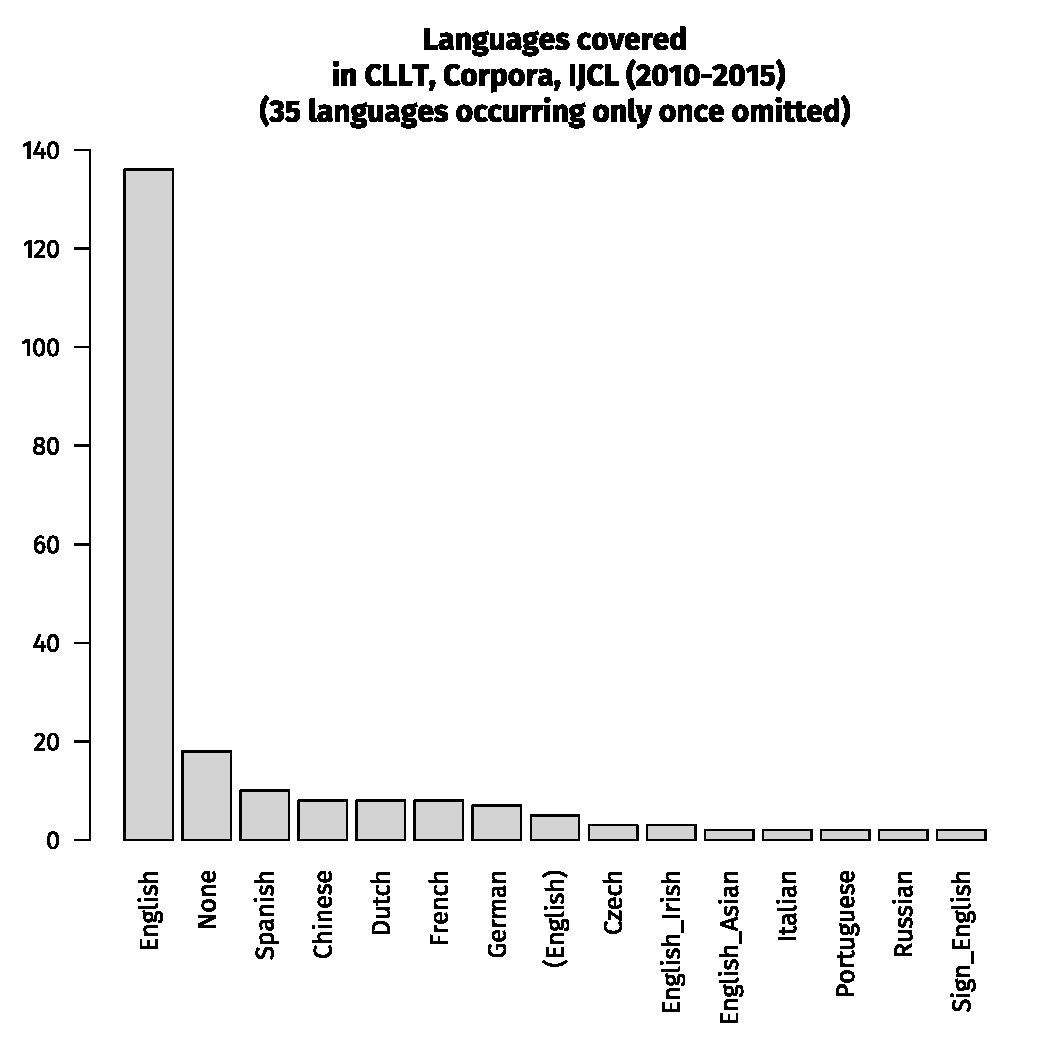
\includegraphics[width=\textwidth]{graphics/langsuse}
  \caption{Languages covered in the three major corpus linguistics journals; \textit{None} was assigned for papers which only address general or theoretical issues without reporting any original empirical work; (\textit{English}) was assigned to papers where English is used for comparison in papers predominantly about other languages; 35 languages which only occurred once are not shown}
  \label{fig:langsuse}
\end{figure}

There is one final point I would like to make right at the outset.\label{abs:survey}
My research on German was mostly published in international journals (such as Corpus Linguistics and Linguistic Theory [CLLT] and Cognitive Linguistics [COGL]).
The international corpus linguistics scene is very active, with at least three major journals (International Journal of Corpus Linguistics [IJCL], Corpora, CLLT) publishing large numbers of papers per year.
In 2016, in preparation for \citet{Schaefer2019}, an open-access introduction to statistical inference and statistical modelling for linguists, I performed a manual annotation of all 198 papers published in IJCL, CLLT, and Corpora between 2010 and 2015.%
\footnote{The raw data will be published with the book.}
The list of languages covered, the corpora used, and the statistical methods used in each paper were annotated.
Figure~\ref{fig:langsuse} shows the distribution of languages (as raw counts).%
\footnote{Since some papers deal with more than one language, 236 language codes were assigned in total.}

English featured prominently in 136 papers (146 if World Englishes and English sign languages are added), followed by Spanish with eleven mentions as a distant second.
German, on the other hand, was a major object of study in only seven papers (four in IJCL, two in Corpora, one in CLLT).
Of course, this does not mean that linguists working on German (or Spanish, Chinese, Dutch, French, etc.\ for that matter) do not use corpora or do not publish their research.
However, this result shows how corpus linguistics as a field is still very much identified with English corpus linguistics (or even BNC linguistics, see Section~\ref{sec:corporaincognitivelyorientedlinguistics}, esp.\ Figure~\ref{fig:corpususe} on p.~\pageref{fig:corpususe}).
While this state of affairs is not detrimental for corpus linguistics, I suggest that corpus linguists working on languages other than English could benefit from taking part in the active theoretical and methodological discussions taking place in international journals.
From my own point of view as a linguist working on German, it seems evident that the German language and German linguistics has a lot to contribute to current debates in corpus linguistics, especially given that German is famous for the probabilistic phenomena labelled \textit{cases of doubt}.
Thus, I hope my work encourages other linguists working on German (and other under-represented languages) to increase the visibility of their object of study in international corpus linguistics for mutual benefit.
While the case studies focus strongly on German grammar, this general introduction predominantly takes up the foundational theoretical and methodological issues.

\newpage

\chapter{Probabilistic grammar}
\label{sec:probabilisticgrammar}

All case studies presented here are empirical explorations of alternation phenomena in the broad sense.
While the term \textit{alternation} is sometimes reserved for syntactic (\ie\ constructional) alternations \citep{Gries2017a}, the four case studies deal with a morphographemic alternation in the context of the development of a new paradigm of the German indefinite article \RDefArt, a morphosyntactic alternation of so-called weak nouns which are gradually shifting towards another declension paradigm \RWeakN, a syntactic alternation between measure noun constructions \RMeasure, and a phenomenon at the syntax-graphemics interface where non-standard punctuation is an obvious indicator of different clausal connections \RWeil.

The nature of an alternation as understood here is that language users have different forms, constructions, or even paradigms at their disposal in a given situation of language production, and that they always make a choice (unless, of course, they decide not to make the utterance).%
\footnote{For the present purpose, I understand \textit{utterance} as comprising events of language production in both the spoken and the written mode.}
While in many cases, prosodic, syntactic, lexical, pragmatic, contextual, and other constraints can be found which account for why speakers tend to choose one form or the other, these constraints appear to be soft and to interact in a weighted fashion, and there often seems to be residual free variation in speakers' choices.
The observable phenomenon is thus clearly probabilistic or stochastic (as opposed to deterministic), and researchers have for a long time acknowledged this fact both for morphological phenomena (see the early overview in \citealt{HayBaayen2005}) and (morpho)syntactic phenomena (see early contributions such as \citealt{Gries2003,Wulff2003,Bresnan2007,Bresnan2007}).%
\footnote{While the number of studies which have produced empirical evidence for the probabilistic nature of morphology and (morpho)syntax is growing, it should be noted that graphemics is under-researched in this paradigm.
Writing is often not viewed as part of grammar or linguistics, and those who do advanced research on writing often view it under an acquisition perspective.
Since I cannot see why phonology and phonetics -- dealing with utterances realised in the spoken medium -- should be treated as part of grammar but graphemics -- dealing with utterances realised in the written medium -- should not (see also \citealt[495--500]{Schaefer2016e}), I extend the probabilistic view to graphemics.
The framework of \textit{usage-based graphemics} was therefore developed by Ulrike Sayatz and me in \ROWeil.
}

While my research clearly stands in the tradition of probabilistic grammar, I want to voice some concerns about the epistemological status of the evidence which we are gathering.
In usage-based and constructionist settings, the type of evidence as found in the papers presented here is often taken as supporting a model of grammar that does without the Chomskyan separation of competence and performance (\citealt{Chomsky1965}; an overview can be found in \citealt[507--518]{Mueller2018}) and\slash or does not embrace an algebraic Aristotelian theory of language in terms of discrete linguistic categories (\eg\ \citealt{Manning2002,Bod2006}; see also \citealt{Kapatsinski2014} for a recent and subjective overview in the same vein).
First of all, doing away with performance altogether is clearly not a reasonable approach considering the body of psycholinguistic research showing how processing constraints affect speakers' and hearers' language use depending on factors clearly not related to learned generalisations (be they stochastic or not).
As \citet[532]{Pullum2013a} puts it,

\begin{quote}
  no sensible grammarian wants or expects grammars to yield direct representations of the raw reality of human linguistic behaviour with all its flubs, false starts and lost trains of thought.
\end{quote}

The core question is rather whether linguistic competence itself is a probabilistic (non-Aristotelian) system (as claimed programmatically by \citealt{Bresnan2007}) or whether probabilistic effects arise from performance alone.%
Another important and only partially related question is whether linguistic knowledge is highly specified, isolated from other forms of knowledge (including linguistic semantic knowledge as distinct from encyclopedic knowledge), and possibly also modular-serial \citep{Fodor1995}, or linguistic knowledge (including semantics) is connected to and (mostly) an indistinguishable part of non-linguistic knowledge (see \citealt{Elman2009}).
While I personally favour a non-Aristotelian view which does not arbitrarily ascribe phenomena to performance, nothing in the data presented in the probabilistic tradition (which includes alternation research) conclusively forces us to assume any specific architecture as is sometimes assumed in usage-based circles \cite{BybeeBeckner2009}.
The traditional division of labour between competence and performance, together with a model-theoretic algebraic theory of syntax including an appropriate probabilistic (constraint-weighting) component, could in principle model all observed effects, including graded acceptability, stochastic alternations, and context-driven effects (\eg\ \citealt[504--507]{Pullum2013}, \citealt{Pullum2013a}, and \citealt[499--500,507--518]{Mueller2018}).%
\footnote{It must be noted, however, that while proponents of model-theoretic syntax often suggest that a probabilistic version is possible \citep[500]{Mueller2018} or even trivial, only few (and often sketchy and inconsequential) attempts have been made to deliver actual implementations (\eg\ \citealt{ArnoldLindarki2007}).}
While some frameworks might make it (apparently) easier to model stochastic effects (sometimes at the cost of coverage or rigidity of formalisation), evidence which decides between theory A -- which assumes highly specific deterministic linguistic knowledge in combination with performance effects and separate from contextual encyclopedic world knowledge -- and theory B -- which favours a stochastic version of linguistic knowledge, not as cleanly separated from encyclopedic knowledge -- is hard to come by.

Interestingly, \citet{Elman2009} (who is on the very far non-Aristotelian end of the Aristotelian vs.\ non-Aristotelian continuum) proposes a radical connectionist model (based on ample experimental evidence and computational models) which does away with the mental lexicon, a component which is in some way, shape, or form part of virtually any linguistic theory in the narrow sense (including stochastic, usage-based, constructionist theories).
In simple terms, Elman proposes a model where words do not have semantic content but merely serve as cues to conceptual and world knowledge.
Despite his comprehensive and erudite argumentation, he admits that the evidence and the computational models are in no way conclusive evidence for his approach \citep[573--574]{Elman2009}.
\citet[573]{Elman2009} states:

\begin{quote}
  However, theories can also be evaluated for their ability to offer new ways of thinking about old problems, or to provoke new questions that would not be otherwise asked.
  A theory might be preferred over another because it leads to a research program that is more productive than the alternative.
\end{quote}

This statement reminds one of the Kuhnian view of \textit{normal science} as a state where a research programme generates enough new and exciting \textit{puzzles} for researchers to solve in order to keep the field alive \citep{Kuhn1970}.
As a matter of fact, the research on alternations and other stochastic phenomena has thrived in frameworks (such as cognitive, usage-based, constructionist linguistics) which try do away (as much as possible) with the competence-performance dichotomy and with a highly modular and specific model of linguistic competence and \textit{not} in generative frameworks (such as Chomskyan minimalism) or model-theoretic frameworks (such as Head-Driven Phrase Structure Grammar), which is why the term \textit{probabilistic linguistics} has become associated with the former type of framework.
My research is therefore presented with reference to usage-based approaches, prominently addressing the prototype vs.\ exemplar debate.%
\footnote{However, it does without a specific commitment to constructionist approaches or cognitive grammar in the narrow sense of \citet{Langacker1987}.}
In a spirit similar to the Jeffrey Elman quote above, I consider the usage-based framework and the associated community the one which currently \textit{offers new ways of thinking about old problems, and which provokes new questions that would not be otherwise asked}, or, in Kuhnian terms, which \textit{offers enough new puzzles to solve} when it comes to stochastic surface effects in language use.
In no way does this mean that I consider the empirical findings intrinsically incompatible with other frameworks.
As soon as people from such frameworks develop a significant interest in modelling my data, they may do so.%
\footnote{Such attempts would be facilitated by the fact that I publish all data related to my published research freely (see \url{https://github.com/rsling}).}

All that said, I see my work less as speaking in favour of any specific linguistic framework and more as making theoretic and above all methodological contributions to some very specific questions, such as the prototype vs.\ exemplar debate (in \RAWeakN, \RAWeil, and \RAMeasure), paradigmatic morphology (in \RADefArt\ and \RAWeakN), graphemics under a usage-based perspective (in \RAWeil), the experimental cross-validation of corpus-derived models (in \RAMeasure).%
\footnote{With respect to the prototype vs.\ exemplar debate, however, a similar situation is described for corpus linguistics in Section~\ref{sec:prototypesandexemplars}.
The data only provide limited cues as to which theory is more appropriate.}
All case studies promote the use of web corpora as ideal sources of data, which is argued for in Section~\ref{sec:corporaincognitivelyorientedlinguistics}.
Finally, the statistical methods used in the analysis of corpus and experimental data are one of my primary foci, which is why Section~\ref{sec:statistics} provides a short overview of statistics and scientific inference.


\newpage

\section{Theories, methods, and data}
\label{sec:theoriesmethodsanddata}

\subsection{Prototypes and exemplars}
\label{sec:prototypesandexemplars}

In this section I discuss one major overarching theoretical theme of the case studies, namely prototype theory and its rival, exemplar theory.
The central question is which type of cognitive representation research on alternations provides evidence for.%
\footnote{This is an extended and modified version of Section~1 from \citet{Schaefer2018} with additions from \citet{Schaefer2016c}.}
The typical approach in alternation research is to annotate a large number of corpus sentences with linguistic features and to model the probability of the variants being chosen given these features.
The idea is that a variant is chosen when the influencing features cumulatively assume typical values for that variant.
For several reasons, a variant of prototype theory with features \citep{Rosch1978} is a good candidate for the appropriate cognitive model.
I will first introduce prototype theory and exemplar theory, including a discussion of the state of the art in linguistics and cognitive science.
The discussion then focusses specifically on the data-driven corpus-based approaches which have been used very prominently in probabilistic modelling and alternation research (see \citealt{Gries2017a}), and whether such approaches have anything to contribute to the prototype vs.\ exemplar debate.

In Aristotelian approaches to linguistic categorisation, category membership is determined by rules and defining features, and it is consequently not viewed as a matter of degree (\citealt{Sutcliffe1993}; \citealt[11--16]{Murphy2002}).
However, based on evidence pointing to the fact that humans often categorise objects by similarity and with varying degrees of fuzziness, prototype theory (\citealt{Rosch1973}; see \citealt{Taylor2008} for an overview) and exemplar theory \citep{MedinSchaffer1978,Hintzman1986} were developed.
Prototype theory assumes that categories are defined by the similarity of their members to a mentally stored abstraction.
This abstraction takes the form of the most prototypical member or -- in later versions of the theory -- weighted features defining the prototype (see \RAWeakN\ for a detailed description of prototype theory with features including \textit{cue validity}).
Many researchers such as \citet{Gries2003,Gilquin2006,NessetJanda2010,Dobric2015} have used prototype theory in some form of corpus-based linguistic modelling.%
\footnote{In the influential framework of cognitive grammar \citep{Langacker1987}, prototypes (which, as should be remembered, represent abstractions already) are literally taken as prototypical exemplars, and there is an additional level of fully discrete abstractions in the form of schemas.
Schemas are characterised by the properties common to all members of the category, whereas a prototypical category member might have very specific additional properties not at all shared by all or even most members \citep[371-375]{Langacker1987}.
The prototype can serve as a reference point when classifying new objects which do not share all properties of the schema, but this would (if repeated) lead to the creation of an even more abstract (hierarchically higher and less specific) schema which describes the new member and the ones belonging to the previous schema.
As pointed out by \citet[136--137]{Langacker1987}, schemas and prototypes thus fulfil different roles and can be assumed to co-exist.
A strict exemplar view of language is incompatible, as far as I can see, with Langacker's view of schemas, but any theory of categorisation that allows for at least some kind of abstraction is not in fundamental contradiction with it.
In my research, I do not use schemas in my descriptions of the relevant categories, mostly because the aspect of similarity and fuzzy classification is central to probabilistic modelling, and a formulation in terms of schemas would bring about an unnecessarily high degree of abstraction (see \citealt[70--71]{Taylor2003} for a parallel argument).}

While prototype theory is well suited for modeling constructional choices, it has a prominent adversary in exemplar theory (\citealt{MedinSchaffer1978,Hintzman1986}).
Prototype theory and exemplar theory model essentially the same types of effects but differ significantly in whether they assume higher-level abstractions in the form of single maximally prototypical exemplars or their features (prototype theory) or assume that categories emerge through the storage of many exemplars and similarity classification on those exemplars (exemplar theory).
\citet{Barsalou1990} already showed that prototype and exemplar theory model the same types of surface effects and are informationally equivalent, at least when it comes to the results of cognitive agents' behaviour.
\citet[84]{Barsalou1990} states that

\begin{quote}
  we can not say whether category knowledge is distributed in exemplars or centralized abstractions.
  But we do know that any account of knowledge that excludes idiosyncratic information, cooccurrence information, or dynamic representation is inadequate.
\end{quote}

Consequently, research producing evidence in favour of one theory or the other commonly does not use mere output data but tests the procedural behaviour of subjects in controlled experiments, for example the speed of category retrieval.
In very early experiments, \citet{PosnerKeele1968} showed, for example, that highly prototypical unseen exemplars were categorised more easily by subjects compared to less prototypical ones which had been included in the data made available to them in order to learn the categories.
This was (at least at the time) taken as evidence that subjects categorise by prototypes.
Since corpus data only show artefacts of production events and we have no experimental access to the speaker's or writer's performance and their actual similarity judgements, one should be sceptical whether corpus analysis alone could ever decide which theory of mental representation is more suitable.
\citet[22]{Gries2003} can be taken as recognising this, when he says:

\begin{quote}
  Frequently, Rosch’s results were [\ldots] interpreted as if they were statements on the structure of mental representations as such; cf.\ the effects = structure fallacy and the prototype = representation fallacy.
  I do not wish to support such interpretations.
  [\ldots]
  Still, even if the form of analysis does not translate into statements on mental representations, the high predictive power [\ldots] shows that the cognitive factors underlying the choice of construction have been identified properly and weighted in accordance with their importance for actual usage.
\end{quote}

A similar caveat (without direct reference to prototypes and exemplars) can be found in \citet[486--487]{Dabrowska2016}, who states that we cannot ``deduce mental representations from patterns of use'', \ie\ from corpus data.\label{abs:dabrowska}
As corpus data are artefacts of cognitive agents' behaviour, they cannot decide between two theories for which Barsalou's informational equivalence criterion holds.

Given this situation, the question arises of how the discussion in the usage-based linguistics community connects with the current discussion in cognitive science.
In cognitive science, it is mostly accepted that exemplar theories have greater explanatory power \citep[184]{Vanpaemel2016} and that abstraction is only needed marginally, if at all.%
\footnote{The hard empirical evidence in favour of exemplar models is substantial.
For example, in \citet{HahnEa2010}, the authors show that subjects even use exemplar similarity over abstract knowledge even when they are given very simple explicit rules to be learned.
This is highly relevant because most other studies focus on the learning of implicit rule-based knowledge, which involves many auxiliary assumptions in actual experiments \citep[2]{HahnEa2010}.
On the other hand, there is evidence that neither theory is fully adequate to model humans' capabilities to form categories.
For example, \citet{ConawayKurtz2016} show that both prototype theory and exemplar theory fail to explain certain experimental results where subjects learn to generalise beyond the input in a way that cannot be explained by similarity.
}
Still, various attempts have been made over the past decades to settle the dispute between abstraction-based models (models with rules or prototypes) and exemplar models, or to find models which unite the two extremes.
\citet{VanpaemelStorms2008} and \citet{LeeVanpaemel2008} proposed the \textit{varying abstraction model} (VAM) which ``attempt[s] to balance economy and informativeness'' \citep[745]{LeeVanpaemel2008}, treating models with full abstraction (radical prototype theory) and no abstraction at all (radical exemplar theory) as special cases of a model which allows for both abstraction and exemplar effects.
The mixture model of categorisation (MMC) by \citet{Rosseel2002} is a model with abstraction in the form of hierarchical clusters of exemplars, and these clusters of objects are characterised by a probability distribution over their features, and categorising new objects is a process of estimating the probability of this object belonging to one of the clusters.
\citet{GriffithsEa2009} go further and present a computational model which is able to choose the appropriate complexity of representation for a given category.
However, despite these (and more) attempts to reconcile or unite the two approaches while developing spelled-out mathematical models, \citet[183--184]{Vanpaemel2016} describes the state of affairs between adherents of neo-prototype theory (such as \citealt{MindaSmith2001,MindaSmith2002}) and exemplar theory as a stalemate.

In cognitive linguistics, \citet{DivjakArppe2013} is a very rare example of a paper where such issues are taken up with reference to the current research in cognitive science.
Their corpus-based approach shows ``one way of systematically analyzing usage data as contained in corpora to yield a scheme, compatible with usage-based theories of language, by which the assumptions of both the prototype and exemplar theories can be operationalized'' \citep[267]{DivjakArppe2013}.
Their approach to implementing a varying abstraction model \citep[254--260]{DivjakArppe2013} is based on hierarchical clustering of annotated properties of sentences.
They cluster sentences containing Russian verbs of trying.
Then, they single out the one sentence from each cluster which scores the highest probability for any of the six \textit{try} verbs according to a polytomous regression model estimated on the same data.
The clusters are interpreted as intermediate-level exemplar-derived abstractions of typical contexts for these high-probability verbs (typically more than one cluster for each verb; \citealt[255--256]{DivjakArppe2013}).
The crucial difference between such data-driven corpus-based analyses and experiments in cognitive science (\citealt{DivjakArppe2013} use \citealt{VerbeemenEa2007} as their reference) is that cognitive research is based on experiments where subjects produce actual category assignments or similarity judgements, and in corpus studies, the categories and category membership are determined purely from existing data.
The experimental approach with reduced and\slash or artificial stimuli makes it much easier to examine very specific effects in the behaviour of the subjects.
While I do not think the results of the case study presented in \citet{DivjakArppe2013} are invalid, any data set can be analysed to yield a certain number of clusters, and this fact alone does not substantiate any claim about one mental representation or another.
Thus, the study does not ensure that the clusters emerging from the data correspond to any speaker's cognitive representation.
In other words, \citet[229--230]{DivjakArppe2013} fall victim to Barsalou's equivalence trap when they state without further motivation that

\begin{quote}
  [t]he objectives of this study are, first, to explore how the prototype and exemplar models of categorization manifest themselves in corpus data [\ldots].
  Although corpus data do not reflect the characteristics of mental grammars directly, we do consider corpus data a legitimate source of data about mental grammars.
\end{quote}

The second sentence of this quote has at least one reading in which it is contradictory.
Compare the (already mentioned) more realistic views in \citet[84]{Barsalou1990}, \citet[486--487]{Dabrowska2016} and \citet[22]{Gries2003}.

As mentioned above, in cognitive science, experimental setups which allow access to the cognitive agents' performance over time are preferred in order to produce evidence for either one of the two competing theories.
See \citet{StormsEa2000} for a comparison of the theories in different experimental settings.
However, the trade-off one has to accept when doing experiments with highly simplified stimuli and very simple tasks is their lower \textit{external validity} (\ie\ their lower degree of generalisability) and their high dependence on potentially problematic operationalisations of constructs, control of confounding factors in the face of a limited number of available subjects, etc. (in other words, critical dependence on \textit{construct validity} and \textit{internal validity}).%
\footnote{Construct validity requires the measurements made in a experiment to be credible and substantive indicators of a theoretically postulated construct (such as a prototype).
Under internal validity an experiment establishes a causal relationship between experimental manipulations and the measured effects through minimisation of systematic measurement error.  
An accessible overview of the different types of validity can be found in Chapter~1 of \citet{MaxwellDelaney2004}.
The discussion of types of validity goes back to \citet{CronbachMeehl1955,CampbellFiske1959}.}
Tasks in cognitive science have been criticised exactly for their lack of external validity, for example by \citet{Murphy2003}.
From a linguistic perspective, it is remarkable in this context that \citet{VoorspoelsEa2011} consider their experimental task -- which is the assignment of typicality scores to nouns from the domains of \textit{animals} and \textit{artefacts} to categories like \textit{bird}, \textit{fish}, \textit{clothing}, or \textit{tools} -- a study of ``superordinate natural language categories, whereas most evidence supporting exemplar representations has been found in artificial categories of a more subordinate level'' \citep[1013]{VoorspoelsEa2011}.
Corpus linguists interested in probabilistic alternation modelling deal with much more complex high-level categories and use large and complex feature sets, especially in (morpho-)syntax.%
\footnote{Notice, however, that recently, approaches have emerged which solve at least some problems by abandoning linguistic high-level features altogether \citep{BaayenEa2016,RamscarPort2016}.
Clearly, they have not (or at least not yet) reached mainstream popularity, and it remains to be seen how well they perform on a broader range of questions.}
It is thus an advantage of much linguistic work on categorisation that it deals with complex and realistically produced data, because this greatly improves the external validity of studies, albeit by sacrificing some construct validity.
An ideal contribution by cognitive corpus linguists to the research on (levels of) category abstraction in the human mind would thus be to provide analyses which have great external validity and complexity while carefully making sure that (and determining to what extent) these finding correlate with reactions from cognitive agents under more controlled experimental conditions, which increases the construct validity.
This is why experimental validations of corpus-derived models should under all circumstances become the standard procedure.
Section~\ref{sec:corporaincognitivelyorientedlinguistics} briefly discusses this approach.

In closing, I want to point out that my work often conveniently uses prototype-theoretical formulations (\RAWeil, \RAWeakN, \RAMeasure) because the high-level contentful features which are mostly used in probabilistic modelling (such as semantic classes of lemmas, definiteness of noun phrases, discourse status, or register, to name just a few) invite a description that allows for abstractions.
However, \ROMeasure\ argues that certain types of effects are at least implausible to model as abstractions.
In the study, it is shown that lemma frequency and construction-lemma attraction influence the choice of alternants.
Such item-specific effects indeed appear to favour an exemplar view.
However, it must be noted that it is always possible that item-specific effects can in fact be traced back to abstraction effects (such as semantic properties of lemmas).
Again, in the spirit of Section~\ref{sec:probabilisticgrammar}, we should be aware that our inferences are more often than not abductive, \ie\ inferences to the (in the view of our research community) best explanation.


%%%%%%%%%%%%%%%%%%%%%%%%%%%%%%%%%%%%%%%%%%%%%%%%%%%%%%%%%%%%%%%%%%%%%%%

\subsection{Corpora in cognitively oriented linguistics}
\label{sec:corporaincognitivelyorientedlinguistics}

\subsubsection{Problems with corpora and some solutions}
\label{sec:problemswithcorporaandsomesolutions}

The empirical analysis of probabilistic phenomena such as alternations requires researchers to make choices with regard to the data they use for their scientific inferences.
Depending on the amount of data available and type of inference, methods for the numerical analysis of the data are also required.
In the present section, I argue why web corpora (\ie\ corpora built using material collected from the WWW) are ideal for the corpus-based work presented here, and I briefly introduce the idea of experimental validation of corpus findings.
Section~\ref{sec:statistics} will then discuss methods of statistical analysis.

Corpora have been used as a major source of data in alternation research and cognitively oriented linguistics in general, and my research is no exception.
Since cognitively oriented linguistics is an attempt to model cognitive representations as well as the cognitive mechanisms involved in using these representations to produce and understand utterances, the question arises whether corpus data -- \ie\ artefacts of language use -- are an appropriate source of data in cognitively oriented linguistics.

Prominently, \citet[591--592]{Gries2017b} argues that corpus linguistics is essentially the quantitative analyses of co-occurrence frequencies (\eeg\ of words and words or words and constructions, words and senses) in collections of texts, which is often related to the \textit{distributional hypothesis} and traced back to \citet{Harris1954}.
Gries also notes that the major tenet of cognitively oriented linguistics is that language users learn language by acquiring knowledge about the probabilities of words, constructions, senses, etc. in a given context (in the broadest sense of the word \textit{context}).
Thus, Gries concludes, both disciplines deal with distributional phenomena and are highly compatible.
Clearly, this is accurate inasmuch as both corpus linguistics and cognitively oriented linguistics examine types of distributional phenomena, but one distributional phenomenon is not necessarily like any other one.
The implicit claim made by Gries is that both fields deal with \textit{the same or at least two highly and causally related distributional phenomena}.
While it is impossible to refute this implicit additional assumption, it is also difficult to substantiate it.
Therefore, I suggest that we accept it as a working hypothesis.
At least, however, the approach begs the question of whether corpora represent the cognitive reality of language users in any meaningful and reliable way.%
\footnote{I do, however, contradict the categorically contemptuous tone found in many works from cognitively oriented linguistics (\citealt[590--593]{Gries2017b} is no exception) against earlier work based on researchers' intuitions.
As \citet{SprouseAlmeida2012,SprouseEa2013} have shown with significant methodological rigour, judgements collected in a traditional way through intuition by linguists can be highly reliable.
The question is rather which types of data are used as evidence to support which claims.
Intuitive judgements (even by linguists) are not intrinsically unreliable; they might just be the wrong tool in certain situations.}
The traditional discussion of the \textit{representativeness} of a corpus does not necessarily help in this context, because it is more often than not centred around the concept of a corpus being \textit{representative of a language} as a whole, using as points of reference:
(i) the distribution of texts or text types in the output of all speakers of a language (production-based),
(ii) the distribution of the relevance of texts or text types in the whole speech community (relevance-based), or
(iii) the distribution of speakers' exposure to different texts or text types (perception-based).%
\footnote{For overviews from different perspectives, see \citet{Biber1993}, \citet{MceneryEa2006}, \citet{Leech2007}, \citet{Hunston2008}.
A summary of the discussion is found in Chapter~5 of \citet{SchaeferBildhauer2013}.}

Indeed, given the argumentation from \citet{Gries2017b} discussed above, a perception-based view of corpora seems to be the most appropriate for a cognitive approach to language where input frequencies play the most crucial role.
However, the linguistic experience of language users is most definitely a highly individual matter, and most corpora force researchers to work with highly problematic abstractions.
In a recent contribution where the percep\-tion-based view is argued to be valid in cognitively oriented corpus linguistics, \citet[104]{StefanowitschFlach2016} take a quite cavalier stance on representativeness:%
\footnote{The picture does not change significantly if corpora are seen as collections of linguistic output events under a cognitively oriented perspective \citep{TummersEa2005}.}

\begin{quote}
In this wider context, large, register-mixed corpora such as the British National Corpus [\ldots] may not be perfect models of the linguistic experience of adult speakers, but they are reasonably close to the input of an idealized average member of the relevant speech community.
\end{quote}

The assumption that an \textit{idealised average speaker} is a valid construct seems naïve at best.%
\footnote{Essentially, they argue for a license to conclude that any distributional pattern found in the BNC automatically has a cognitive reality.
If life were this easy, many more researchers would certainly use the BNC exclusively.}
If the concept of an idealised average speaker were admissible and if there were indeed corpora (like the BNC) representative of this idealised speaker's input, then different actual speakers should not learn considerably diverging grammars.
If it turns out that actual speakers indeed acquire fundamentally different grammars, however, then the idealisation is unwarranted.
There is growing evidence from both psycholinguistic research and cognitively oriented linguistics that differences between competent adult speakers of a language are substantial and should not be averaged.
This concerns speakers' performance in linguistic tasks (\citealt{HuettigJanse2016} and references therein), but it also affects their individual grammars.
For example, \citet{Dabrowska2008,Dabrowska2012} clearly found that there is no convergence of the grammars of different Polish adult speakers towards a unified grammar (with respect to the phenomena under study), and \citet{Dabrowska2015} puts this into a larger picture.
This does, of course, not entail that speakers would perceive each other's languages as \textit{different} like foreign languages or dialects -- or that they would be expected to have problems communicating in their everyday life.
However, this clearly questions the usefulness of the concept of an \textit{idealised average speaker}.
A commonly adopted solution is to model speaker-variation as a nuisance variable, usually by adding a per-speaker random effect to the statistical models (\citealt{Gries2015}; \citealt{Schaefer2018}; see Section~\ref{sec:statistics}).
Most corpora, however, lack metadata to identify the authors of specific texts reliably.
If they do, single authors usually contribute far too few data to take individual variation into account in an informative way.
But even if there are enough data, the random-effect approach is just a way of taking care of unmodelled heterogeneity (see also Section~\ref{sec:modeleverything}).
It does not make the remaining \textit{averaged} part of the model more cognitively real.%
\footnote{Although without specific empirical backup, \citet[695--698]{Newmeyer2003} already made this point convincingly, which is something one can admit without committing to the full argument he put forward.}

In the corpus linguistic discussion on representativeness (as mentioned above), this problem has received little attention, mostly because this discussion has traditionally focussed on a global notion of representativeness.
An ideal corpus of a language is assumed to be representative of a language (such as English or German) as a whole (whatever that means).
This holistic approach to the question of representativeness (which surely still inspired the view argued for by \citealt{StefanowitschFlach2016}) is not applicable to cognitively oriented linguistics, which probably requires techniques for experiments and observational studies similar to those in the social sciences, psychology, and cognitive science.
The goal in scientific experiments (or scientific studies, to use a more general term) is to make inferences about a \textit{population of interest} using a sample of data from that population.
The population of interest has to be defined with regard to each experiment individually, and it might be something very specific (such as the written output of speakers of a certain age, in a specific register, etc.) instead of \textit{the language} or \textit{the average speaker} (across all communicative settings and modes).
In the social sciences, the concepts of \textit{global and specific representativeness} \citep[86]{Bortz2005} are used to describe the relevant distinction.
The crucial point is thus not whether a corpus is \textit{representative of a language} but whether a sample taken for a specific purpose represents the population of interest for the concrete study.

A standard approach implicitly adopted in many corpus studies (including mine) is to define the population of interest as \textit{corpus exemplars in which a certain range of constructions, words, etc.\ occurs}.%
\footnote{This implicitly assumes something similar to what \citet[27]{BerkFreedman2009} call an \textit{imaginary population}.
Their criticism applies only in limited ways to corpus sampling given the argument I make here.}
This is effectively what we do if we run unrestricted queries looking for specific morphological or syntactic patterns in some large corpus like the DeReKo of the Institut für Deutsche Sprache (IDS; \citealt{KupietzEa2010}) or the DECOW16A \citep{SchaeferBildhauer2012,BiemannEa2013,SchaeferBildhauer2013,Schaefer2015b}.
With certain caveats taken into consideration and given the right research question, nothing speaks against this approach, as I will argue below.
Going beyond this unrestricted query approach, however, \citet{Gries2015,Gries2017b} argues that by using metadata (as available for the British National Corpus; \citealt{Lee2001,Burnard2007}), searches can be refined to specifically examine phenomena with different (relative) frequencies in different modes, genres, etc.
If there is no hypothesis that mode, register, etc. have an influence on (relative) frequencies, however, such refinements are not strictly required.%
\footnote{Note that the word \textit{influence} implies a \textit{causal relationship}.}

The unrestricted query approach works when the hypothesis is that the relative frequencies of two structures A and B change when going from condition x to condition y.
Mathematically, this hypothesis can be expressed as (\ref{eq:001}) (see also Section~\ref{sec:nevereverrandomfallacy}).%
\footnote{f(A|x) is to be read as in the notation for conditional probabilities, except with frequencies instead of probabilities.
  It is thus the \textit{frequency of item A under condition x}.}

\begin{equation}
  \frac{f(A|x)}{f(B|x)}\not =\frac{f(A|y)}{f(B|y)}
  \label{eq:001}
\end{equation}

For example, in \ROWeakN\ one hypothesis was that the frequency of the singular non-nominative form of a weak noun such as (\textit{den}\slash\textit{dem}\slash\textit{des}) \textit{Planeten} `planet' (structure A) compared to the frequency of its (non-standard) strong form (\textit{den}\slash\textit{dem}\slash\textit{des}) \textit{Planet} (structure B) is different in the genitive (condition x) than in the accusative and dative (condition y).

As long as a corpus contains both structures and \textit{given the randomness assumption} (RA), the hypothesis can be examined using an unrestricted query.
The RA holds if all other potential influencing factors which favour the occurrence of A or B are distributed equally in the conditions x and y.
In the example, individual lemmas might have a tendency to favour the strong form over the weak form or vice versa, or different registers might favour one form over the other etc.
However, given a random assignment of lemmas, registers, and so on, condition x and condition y would always yield a different distribution of A and B under hypothesis (\ref{eq:001}).
The RA could thus still hold even if the strong (non-standard) form occurred predominantly in a specific register or mode, and if (additionally) the corpus did not contain very many texts from this register or mode.%
\footnote{In the given example, this might be the case with the DeReKo.
It contains predominantly edited newspaper texts, and the strong forms -- being non-standard -- are probably very rare in such texts.}
However, effects might be more difficult to detect in such a situation; see Section~\ref{sec:nevereverrandomfallacy} for more on this.
In the worst case, a corpus might simply contain not enough exemplars of a certain phenomenon as a result of an inappropriate register or mode composition.
This would be detrimental for any study, but it is also definitely not related to the RA.
In any case, problems with the RA are not exclusive to linguistics or corpus linguistics, but represent standard problems with data sampling for experiments.%
\footnote{``Drawing a random sample of the U.\,S.\ population, in this technical sense, would cost several billion dollars (since it requires a census as a preliminary matter) and would probably require the suspension of major constitutional guarantees. Random sampling is not an idea to be lightly invoked.'' \citep[23]{BerkFreedman2009}}

On the basis of these elaborations, I propose that the core problem for corpus studies in cognitively oriented linguistics is not the RA.
Rather, it is one of the following problems (depending on the research question):

\vspace{\baselineskip}

\begin{itemize}
  \item\label{it:pooled} \textbf{Problem 1}: The corpus contains pooled output data from numerous individual speakers, making it impossible or difficult to draw conclusions about cognitive representations (see \citealt{Dabrowska2008,Dabrowska2012,Dabrowska2015}).
  \item\label{it:meta} \textbf{Problem 2}: The corpus does not contain the relevant meta-information to draw a sample which represents the population of interest in a given study (for example, if genre or register effects are of interest and the corpus does not contain the relevant metadata).
  \item\label{it:composition} \textbf{Problem 3}: Even if the composition of the corpus in terms of registers, modes, etc.\ is not a primary research interest, a phenomenon which occurs only in specific registers, modes, etc.\ might be underrepresented in a given corpus because of its composition.
\end{itemize}

\vspace{\baselineskip}

\textbf{Problem~1} has multiple remedies.
At first sight, it might seem a valid option to enrich corpora with metadata such that the writer\slash speaker of each exemplar can be identified, then taking per-speaker preferences into account (as promoted by \citealt{Gries2015,Gries2017a}).
However, if the mental grammar of each speaker varies (as suggested by \citealt{Dabrowska2008,Dabrowska2012,Dabrowska2015}), then it would not be sufficient to take per-speaker \textit{tendencies} into account in the sense of: \textit{speaker i favours variant A over variant B with probability $p_i$}.
Instead, a separate (statistical) model (or a complex model with per-speaker random slopes) would have to be built for each speaker, since the influencing factors guiding each speaker's grammatical choices would be weighted differently.
This would lead either to extremely complex over-parametrised models (if random intercepts and slopes are used; see Section~\ref{sec:statistics}) or to a lot of different models with no way to come up with an interesting generalisation.
\citet{KupermanBresnan2012} suggest (in the context of an experimental setting) to use multi-model averaging \citep{BurnhamAnderson2002} to take into account the variation between speaker-grammars (see also \citealt{BarthKapatsinski2014}).
While this might be applicable for psycholinguistic experiments, it is clearly not feasible in corpus studies with large numbers of speakers, especially since the models over which one averages should be known theoretical options.
In any case, the per-speaker data would be too sparse in any conceivable corpus to make such over-parametrised modelling feasible.

Another more realistic option is to focus on the cognitive principles that theories of cognition predict should govern the formation of mentally represented grammars.
Such cognitive principles should be observable with considerable stability across groups of speakers.
In \ROWeakN, for example, I used predictions derived from \citet{Koepcke1995} about the prototype representations of weak nouns (in the sense of inter-individual cognitive principles) to derive predictions for the outcome of the corpus study.
In \ROMeasure, I used arguments from grammaticalisation research \citep{Koptjevskaja2001} to argue for plausible general cognitive mechanisms which guide the relevant choice between two pseudo-partitive NP structures.
Based on such assumptions, the use of massively pooled data from large corpora is not unjustified, and it avoids the dangers of data dredging and fishing for spurious correlations \citep{GoodHardin2012}.
Even under the assumption of such theoretical predictions about general cognitive mechanisms, it should become standard practice to evaluate corpus-derived models using experimental techniques to check whether corpus data and reactions by native speakers under controlled conditions converge.
A review of the state of the art was provided by \cite{NewmanSorensenduncan2015}, who enumerate a number of studies showing how corpus data and experimental data converge (such as \citealt{BresnanEa2007,DurrantDoherty2010,GriesWulff2005,GriesEa2005}) and a number of studies where the two types of data led to diverging or only partially converging results (such as \citealt{ArppeJaervikivi2007,Dabrowska2014,Mollin2009}).
When researchers do not achieve convergence, they often try to explain this by differentiating between the actual cognitive construct and whatever the pooled usage data as found in corpora represent.
For example, \citet[411]{Dabrowska2014} lists a number of possible reasons to explain why subjects in her experiment diverged in their word association preferences from collocation measures extracted from corpora.
Alternatively, researchers argue for a more adequate statistical analysis to increase the fit between corpus data and experimental data.
See, for example \cite{DivjakEa2016}, who show that generalised additive models (GAMs) are better suited than generalised linear models (GLMs) for correlating reading times and corpus data. 
No general consensus and no commonly accepted best-practice approach has emerged so far, which is not surprising given the number of cognitive constructs assumed at diverse levels, the problems of corpus composition, the operationalisations involved in experiments, and the choice of statistical tools.
Also, experimental validation of corpus-based findings has simply not become a general requirement.
As \citet[3--4]{DivjakEa2016a} put it:

\begin{quote}
  There are now a number of published multivariate models that use data[,] extracted from corpora [\ldots] to predict the choice for one morpheme, lexeme or construction over another.
  However, [\ldots] only a small number of these corpus-based studies have been cross-validated [\ldots].
  Of these cross-validated studies, few have directly evaluated the prediction accuracy of a complex, multivariate corpus-based model on humans using authentic corpus sentences [\ldots].
\end{quote}

Therefore, in \ROMeasure, I used experimental validation in two different paradigms and provide possible explanations for the quality of the fit between the corpus data and the experimental data, much in the spirit of \citet{Dabrowska2014}.%
\footnote{See also \citet{SchaeferPankratz2018}, where a different type of experimental validation of corpus-based findings is used.}

Turning to \textbf{problem~2}, there is a relatively simple solution in theory, which might, however, be difficult to implement in practice.
If the corpus lacks the appropriate metadata, one can simply draw an unrestricted sample and manually annotate the relevant registers, styles, etc.\ afterwards.
While this might sound quite laborious, it also ensures that the relevant categories are the ones the researcher has a theory-driven hypothesis about.
Given the many different definitions of registers and similar categories, it is not likely that corpus creators would annotate a corpus with exactly the taxonomy the researcher has in mind.%
\footnote{Also notice that recent approaches to automatic large-scale register identification failed with a classification accuracy in the region of 50\% \citep{BiberEgbert2016}.}
Of all of my studies collected here, only \ROMeasure\ made reference to style (not register) as an influencing factor.
Fortunately, as one of the creators of the DECOW corpora, I could implement the necessary technology to automatically annotate the corpus with proxy variables to style (see \RAMeasure, also \citealt{SchaeferEa2013}).

Finally, \textbf{problem~3} has a relatively simple solution.
Under the unrestricted query approach (which -- I want to stress once again -- was used for all research collected here), data sparsity can be remedied by creating larger and at the same time more varied corpora.
Research on phenomena which are simply rare in general benefit from sheer corpus size.
In all case studies collected here, one of the examined variants had a low frequency, and the studies all benefitted from the fact that the corpus used (DECOW in different versions) was very large.
In \ROWeakN, the proportion of forms of the weak nouns inflected according to the strong paradigm was reported to be between approximately 1\% and 2\%.
In \RODefArt, the forms of the cliticised indefinite article was estimated to account for roughly 2.5\% of all forms of the indefinite article.
Furthermore, in \ROWeil, clauses headed by \textit{obwohl} `although, then again' and \textit{weil} `because' showing verb-second order made up roughly 6\% to 7\% of all clauses headed by those particles.
Only in \ROMeasure\ was the situation less extreme, with the rarer of the two competing measure NP constructions accounting for approximately 22\% of all exemplars in the sample.

Furthermore, DECOW is a web-derived corpus created by an unrestricted crawl of the German-speaking web.
As such, it contains documents written in all sorts of styles, registers, and text types.
These include sources of non-standard written language such as forums, which is not true of the other very large German corpus, the DeReKo.
The fact that such sources are included in the corpus was vital for at least \RODefArt, \ROWeakN,  and \ROWeil\ because the relevant alternation is only truly productive in non-standard language, as normative grammars ban one of the alternants.%
\footnote{Some normative grammars take similarly clear stances on the phenomenon discussed in \ROMeasure, as pointed out in the paper.
However, the normatively dispreferred variant is still used quite often, despite such attempts to suppress it.}
With any other available corpus, the case studies would have run into problem~3 (data sparsity due to an inappropriate composition of the corpus in terms of registers, modes, text types, etc.).
In Section~\ref{sec:webcorpora}, I therefore provide a short motivation of why web corpora are an important new source of data.

\subsubsection{Web corpora}
\label{sec:webcorpora}

Web corpora were made popular through the WaCky initiative \citep{BaroniEa2009} starting around 2005.
The WaCky corpora were attractive to many researchers because they were made available freely and could be downloaded fully, which allows for all kinds of local processing not possible through web-based query interfaces.
In parallel, the SketchEngine corpora were developed as a commercial alternative \citep{KilgarriffEa2014}, and the SketchEngine project probably represents the most significant current provider of web-derived linguistic corpora.
The COW corpora have been under development since 2012 \citep{SchaeferBildhauer2012,SchaeferEa2013,SchaeferBildhauer2013,Schaefer2015b,BildhauerSchaefer2016,Schaefer2016a,Schaefer2017,BildhauerSchaefer2017}.
Like the WaCky corpora, they are freely available both for download and via a web interface for easy querying.%
\footnote{\url{https://www.webcorpora.org/}}

While smaller specialised corpora are sometimes derived from web data (\eeg\ \citealt{Krause2016}), the major advantages of web data in the context of the research presented here (see especially problem~3 from Section~\ref{sec:problemswithcorporaandsomesolutions}) is that there is a virtually unlimited supply of textual data available on the web.
Also, web data includes non-standard written forms, and the breadth of the variation contained within it is enormous.
For example, in \citet{BildhauerSchaefer2016,BildhauerSchaefer2017}, it was shown that the DECOW16 web corpus has a much broader spread of topics than the DeReKo newspaper corpus.%
\footnote{Additionally, a large-scale analysis of the distribution of automatically extracted lexico-grammatical features in web documents and the DeReKo corpus is being prepared for publication by the Institut für Deutsche Sprache and the present author.}

Thus, web corpora were the obvious choice for the case studies, and the DECOW corpus was created by me specifically for the purpose of conducting my linguistic research published between 2014 and today.%
\footnote{This is not the place to discuss technical details of web corpus construction.
  \citet{SchaeferBildhauer2013} provides a convenient introduction to the subject.}
Given the data from the survey to be published in \citet{Schaefer2019} (see p.~\pageref{abs:survey}), we can assess the impact web corpora have had on current research in corpus linguistics by looking at the frequency with which different corpora have been used in research published in the three major international corpus linguistics journals between 2010 and 2015.
Figure~\ref{fig:corpususe} plots the distribution of the corpora used (328 usages of corpora in 198 papers).

\begin{figure}[htpb]
  \centering
  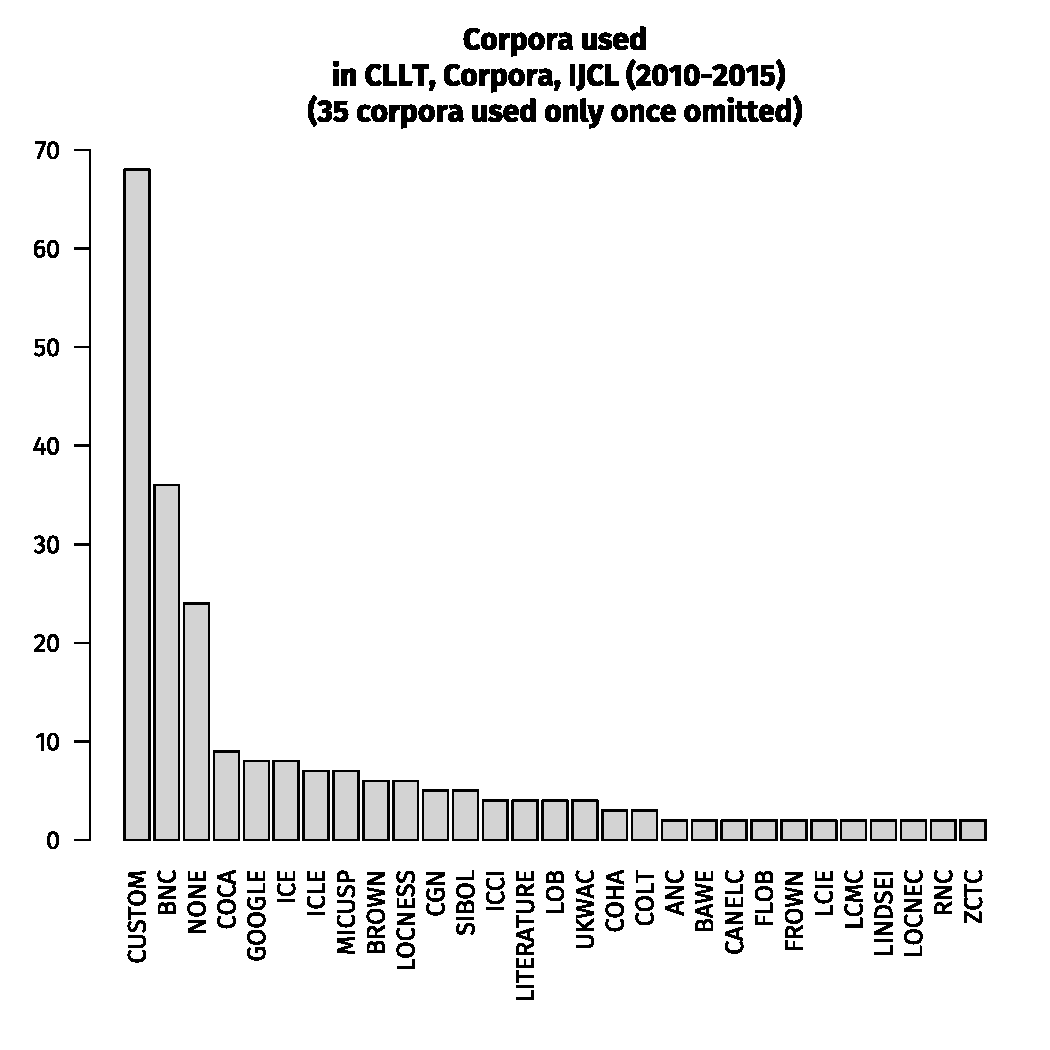
\includegraphics[width=\textwidth]{graphics/corpususe}
  \caption{Corpora used in the three major corpus linguistics journals; CUSTOM was assigned when authors reported the creation of a custom corpus for the concrete study (a selection of newspaper articles, of academic papers, etc.); LITERATURE was assigned to papers about specific literary works; 111 corpora which were only used once (including DeReKo) are not shown}
  \label{fig:corpususe}
\end{figure}

Figure~\ref{fig:corpususe} clearly shows that the distribution of the use of corpora follows almost a power law distribution.
Custom corpora built for a specific research project are most frequent (used 68 times), followed by the BNC (used 36 times) and a distant third, the COCA (nine times).%
\footnote{I do not even begin to discuss the problems of reproducibility involved when a custom corpus is created ad-hoc for a single research paper.
The problem is even graver when web data is used in an ad-hoc fashion for corpus creation or even gathered by googling \citep{Kilgarriff2006}.}
The English UKWAC web corpus was used only four times, and the French FRWAC and the German DEWAC were each used once.
Given the advantages of web corpora as argued for above, this is a baffling result.
Before turning to an in-depth view of statistical methods used in my research, I therefore wish to point out that web corpora clearly seem to be underused in contemporary corpus linguistics.
I hope the case studies presented below demonstrate their usefulness and inspire other corpus linguists to use them in their research.

%%%%%%%%%%%%%%%%%%%%%%%%%%%%%%%%%%%%%%%%%%%%%%%%%%%%%%%%%%%%%%%%%%%%%%%

\subsection{Statistics}
\label{sec:statistics}

\subsubsection{Overview}
\label{sec:methods:overview}

This section is exclusively about statistical modelling, which is often seen as an indispensable part of probabilistic modelling \citep{Gries2017b}.
Subsection~\ref{sec:onstatisticalinference} briefly describes known problems with inferential statistics as used by many practitioners.
Subsection~\ref{sec:nevereverrandomfallacy} discusses how certain problems with what is called the \textit{non-randomness of linguistic data} do not affect many types of statistical analysis.
Directly related to the previous subsection, Subsection~\ref{sec:modeleverything} addresses problems with the associated idea that statistical models must always be exhaustive.
Finally, Subsection~\ref{sec:bayesianhype} briefly shows that Bayesian modelling (as sometimes advocated for these days) usually will not lead to different results.


\subsubsection{On statistical inference}
\label{sec:onstatisticalinference}

In this section, I briefly discuss my position on data analysis and so-called \textit{hypothesis testing}.
The most widely used statistical system is \textit{Null Hypothesis Significance Testing} (NHST), and it is one of the \textit{frequentist} systems of statistical inference.
In NHST, researchers attempt to substantiate the existence of an effect (such as a positive connection between the three different non-nominative cases on an NP and the occurrence of a non-standard form in the NP, see \RAWeakN) which is predicted to exist by their favoured theory by means of conducting an experiment in which the effect is measured.
Then, the probability $p$ (the so-called \textit{p-value}) of obtaining the observed measurements or more extreme measurements under the assumption that there is actually \textit{no} effect (the \textit{null hypothesis} or just the \textit{null}) is calculated.
If this probability is lower than a certain threshold (usually called the $\alpha$-\textit{level}), the null hypothesis is \textit{rejected}, which is taken as evidence that the hypothesis derived from the theory is correct.
It is often incorrectly stated that \textit{the experiment\slash test shows that the probability that the null is correct is $p$} or \textit{is lower than $\alpha$}.
This approach is riddled with philosophical and statistical problems and has led to the promotion of of bad scientific practice.
Among the most ardent critics are \citet{Gigerenzer2004}, \citet{Colquhoun2014}, and \citet{MunafoEa2017}.
The editors of the journal \textit{Basic and Applied Social Psychology} have even banned the use of p-values in an actionist attempt to tackle problems of bad science related to NHST \citep{TrafimowMarks2016}.
Critics often propose to abandon frequentist inference altogether and adopt a Bayesian approach, which itself is not without philosophical and practical problems (see, for example, \citealt{Mayo1996}, \citealt{Senn2011}).
Others have proposed abandoning statistical inference proper in favour of confidence intervals and effect sizes \citep{Cumming2014}, sometimes not noticing that NHST confidence intervals are not considerably different from NHST p-values, as \citet{Perezgonzalez2015b} shows in reply to \citet{Cumming2014}.

However, there is no need to abandon frequentist inference or p-values simply because they have been abused.
A great many statisticians and researchers have shown that the major problem with NHST is that it is a mixture of the statistical philosophies of Ronald A. Fisher on the one hand and Jerzy Neyman and Egon Pearson on the other hand (see \citealt{Goodman2008}, \citealt{Perezgonzalez2014}, \citealt{Perezgonzalez2015}, \citealt{GreenlandEa2016}; see also \citealt{Lehmann1993} and \citealt{Lehmann2011} for an overview of these two philosophies and the history of their development).
I follow Fisher's statistical philosophy, and I briefly compare it to Neyman and Pearson's now.

Neyman and Pearson developed a system where two hypotheses are specified:
the \textit{main hypothesis} (H\Sub{M}) and the \textit{alternative hypothesis} (H\Sub{A}).
These hypotheses have to exhaust the probability space such that $p(H_M\cup H_A)=1$.
The goal is to accept either of these hypotheses and reject the other, where typically H\Sub{M} is the hypothesis predicted by the experimenter's favoured theory and the one they would like to accept.
The reason why the Neyman-Pearson approach can be hard to implement is that H\Sub{M} needs to be specified \textit{precisely}, \ie including the effect size.
For example, if the experiment is a reading time experiment contrasting reading times under two distinct conditions, then the expected increase in reading times needs to be specified numerically.
If this is possible, researchers can calculate the risk of incorrectly accepting H\Sub{M} when it is false ($\alpha$) and the risk of incorrectly accepting H\Sub{A} when it is false ($\beta$) \textit{given specific sample sizes}.
Then, researchers can decide upon the optimal sample size and choose the optimal testing procedure.
Especially Neyman designed this system explicitly with the idea in mind that researchers end up doing the right thing in $1-\alpha$ of all cases if they follow this protocol.
No inference with respect to the ultimate truth of a specific hypothesis at hand was ever intended by Neyman, and all he wanted to achieve was long-run control of error rates.%
\footnote{\citet{Mayo1996,MayoSpanos2004,MayoEa2009,Mayo2018} propose a theory of statistical inference (called \textit{severe testing}) which is similar to the Neyman-Pearson system, but which also allows inferences about the case at hand.
Unfortunately, severe testing is mostly uncharted territory for practitioners in most fields, including linguistics.}
I refer to this quote from \citet[290-291]{NeymanPearson1933} on hypothesis testing:

\begin{quote}
  We are inclined to think that as far as a particular hypothesis is concerned, no test based upon a theory of probability can by itself provide any valuable evidence of the truth or falsehood of a hypothesis.
\end{quote}

Similarly, \citet[349]{Neyman1937} has this to say about frequentist confidence intervals (italics in the original):

\begin{quote} 
  It will be noticed that in the above description the probability statements refer to the problems of estimation with which the statistician will be concerned in the future.
  In fact, I have repeatedly stated that the frequency of correct results \textit{will} tend to $\alpha$. [fn.\ omitted, RS]
  Consider now the case when a sample, $E'$, is already drawn and the calculations have given, say, $\underline{\theta}(E')=1$ and $\bar{\theta}(E')=2$.
  Can we say that in this particular case the probability of the true value of $\theta_1$ falling between $1$ and $2$ is equal to $\alpha$?
  The answer is obviously in the negative.
  The parameter $\theta_1$ is an unknown constant and no probability statement concerning its value may be made [\ldots] .
\end{quote}

In empirical linguistics (both corpus-based and experimental), following the Neyman-Pearson protocol is often impossible because theories do not predict effect sizes and\slash or no previous knowledge exists about the expected effect size.

Fisher developed a different system, in which the probability of a specific outcome (or a more extreme outcome) of a random experiment \textit{if there is no effect} (the H\Sub{0} or \textit{null hypothesis} or simply the \textit{null}) is calculated as the p-value.
It cannot be stressed enough that this is the probability of obtaining such results \textit{before the experiment is conducted}, and that it is \textit{conditioned on the design of the experiment}.
It is \textit{not} a Bayesian posterior probability which allegedly quantifies the credibility of a hypothesis given the data.
Changing the experiment design changes the sample space and thus leads to different frequentist probabilities, even if the actual measurements are the same.
Therefore, unrealised events play a role in the frequentist interpretation of experiments.%
\footnote{This is seen as a problem by some statisticians and researchers who favour the likelihood principle (and Bayesian inference) over frequentism \citep{Birnbaum1962}.
See \citet{Mayo2014} for a summary of the defense of frequentism against likelihoodism.}

Now, \citet[504]{Fisher1926} suggests an informal, adaptive, and approximate \textit{threshold of significance} (or \textit{sig}), for example $0.05$, below which researchers might suspect that there is something going on.
While Fisher did not recommend the direct inspection or interpretation of p-values (at least not until very late in his life; see Section~4.4 of \citealt{Lehmann2011}), he recommended that experimenters set \textit{sig} appropriately based on previous experimental or theoretical knowledge.
The most important pitfalls and misunderstandings (directly translating into some of the false assumptions common in NHST) in Fisher's framework are:

\vspace{\baselineskip}

\begin{enumerate}
  \item \label{it:fisher00} Researchers think that the p-value corresponds to the posterior probability (called the \textit{inverse probability}; see \citealt{Senn2011}) that the null hypothesis is true.
  Or, even worse, they believe that the posterior probability that the substantive hypothesis is true is $1-p$.
  \item \label{it:fisher01} Researchers take a significant result as a \textit{proof} of something, usually the hypothesised effect.
  In fact, significance only shows that either the null does not describe the actual world very well \textit{or a rare event has occurred}.
  There is no way of knowing with any specifiable accuracy which of these is the case.
\item \label{it:fisher02} Practitioners take point~(\ref{it:fisher01}) even further and make an inference from a single significant result to some substantive hypothesis such as \textit{my whole theory is correct}, forgetting that the test evaluates not just the theory, but also the adequacy of the experimental setup, the accuracy of the measurements, the operationalisations used to measure a theoretical construct, etc.
  \item \label{it:fisher03} Researchers assign high importance to some significant result and low importance to post-hoc effect size.
    This leads to overly optimistic interpretations of the data when they suggest that the null might be rejected ignoring that the effect is actually rather small.
  \item \label{it:fisher04} If one runs a series of experiments and performs the corresponding tests in which the nulls are conceptually related, the actual probabilities of a rare event happening increase, and each $p$ or the \textit{sig} level are too optimistic if left uncorrected.
\end{enumerate}

\vspace{\baselineskip}

Point~(\ref{it:fisher00}) has been addressed ad nauseam by statisticians and statistics-aware practitioners (see \citealt{Goodman2008}, \citealt{Perezgonzalez2014}, \citealt{Perezgonzalez2015}, \citealt{GreenlandEa2016}).
It is simply not true that frequentist p-values contain any information about the probability that any hypothesis is true given the evidence.
The p-value (in Fisher's system, where p-values have a proper definition) is the probability of the outcome of the experiment (or a more extreme outcome) under the null \textit{before the experiment was conducted}.
After the experiment has been conducted, the outcome (however unlikely it might have been before the dice were rolled) is obviously factual and therefore has a probability of 1 like all other facts.

Points~(\ref{it:fisher01}) and~(\ref{it:fisher02}) can be remedied by researchers being aware of the (relatively) low importance which should be attributed to a single significant result.
Furthermore, good use of previous experimental and theoretical knowledge in evaluating the actual p-values (although Fisher himself was not much interested in interpreting them) helps to make the Fisher approach more sound in practice.
It also helps to do replications and perform meta-analyses.
Problems with point~(\ref{it:fisher03}) are easily avoided by looking at post-hoc effect sizes.
Fisher used the informal notion of \textit{sensitivity} to alert practitioners that if, for example, a weak effect is detected with a very large sample, the result might not mean very much despite a successful rejection of the null.
Demanding that researchers pay more attention to effect sizes is really just another way of saying that they should do proper exploratory\slash descriptive analysis of their data sets.
Point~(\ref{it:fisher04}) can be dealt with by applying corrections for group-wise error (which should not be called \textit{$\alpha$-level correction} under Fisher's approach, even if the two are mathematically equivalent).

One objection against Fisher-type statistical inferences comes from the underlying randomness assumption (see the second chapter of \citealt{MaxwellDelaney2004} for a very accessible introduction to Fisher's ideas about randomness).
Fisherian statistical inference is only valid if the randomness assumption (RA; see above in Section~\ref{sec:problemswithcorporaandsomesolutions}) holds.
If practitioners do not conduct a proper random experiment (wilfully or out of ignorance), they are changing the sample space and thereby invalidating the actual computations of the statistical tests.
This was addressed in a prominent paper on statistics for corpus linguistics, and the next section discusses this problem.

\subsubsection{Language is never ever random?}
\label{sec:nevereverrandomfallacy}

In \citet{Kilgarriff2005}, Adam Kilgarriff made an interesting argument about corpora, statistics, and the RA.
In this section, I briefly review the most important points of his argument and propose (in a point-by-point fashion) that the problems mentioned by Kilgarriff do not affect the type of research presented here more than any empirical science.

First of all, Kilgarriff points out that the relation between two types of events (such as the occurrences of two lexemes next to each other in a corpus) can be one of the following (with my paraphrases of the terms' interpretations).

\vspace{\baselineskip}

\begin{itemize}
  \item \textbf{random}\\
    completely uncorrelated
  \item \textbf{arbitrary}\\
    co-occurring without an underlying causal relationship
  \item \textbf{motivated}\\
    co-occurring because of an underlying causal relationship
  \item \textbf{predictable}\\
    standing in a causal relationship where one event is a sufficient condition for the other
\end{itemize}

\vspace{\baselineskip}

The strength of the link between events standing in these types of relationships to one another obviously increases from top to bottom.
Kilgarriff explains correctly that significance testing is only able to discern between a situation of randomness (R, the situation under the assumption of the null hypothesis) and non-randomness (¬R).%
\footnote{Kilgarriff consistently uses the term \textit{NHST} without making it clear whether he means NHST in the narrow sense described above or Fisherian inference.
It appears clear to me that he does not have Neyman-Pearson error control in mind.}
Whenever two types of events do not stand in a random relationship to one another (such as weak nouns occuring more often in a strong form when the NP has dative case compared to when it has genitive case, see \RAWeakN), no statistical system (including Bayesian statistics) can help us to decide whether the correlation is arbitrary (or \textit{accidental}, to use a less precise colloquiual term) or motivated, \ie\ causal.
While Kilgarriff is absolutely right in pointing this out, the situation is exactly the same in any science.
This is why hypotheses are usually chosen with great care and based on sophisticated theories (see \citealt{Chalmers2013} for an introduction, especially chapters~5--7).
It is essential to test only substantive hypotheses and give the test the best and toughest chances of finding errors in the theory which generated the hypotheses.
In other words, while Kilgarriff is entirely right, it is also completely unjustified to expect statistics to do the job that theory and experiment design usually do.
To illustrate this point further, Kilgarriff's example goes like this:
A study might find that shoe polish and cat food are bought simultaneously significantly more often than to be expected under the null (\ie\ given the number of times the items are bought).
A statistical test might reject the null, which states that \textit{the probability of shoe polish being bought when cat food is also bought is the same as the probability that shoe polish is bought when no cat food is bought}.
However, we would have no reason to assume that the relationship between the two types of events would be anything but arbitrary, although it would be very likely not random.
He argues that this could be accounted for if both articles are more often bought together for independent reasons during hot weather or something along those lines.
The point is that any researcher who would conduct such an experiment \textit{without a substantive theory-driven hypothesis} about why buying shoe polish and buying cat food should be correlated has already engaged in bad science, and frequentist statistics cannot be blamed for this.

A second major point raised in \citet[266]{Kilgarriff2005} is that

\begin{quote}
  [w]hether we can reject the null hypothesis [\ldots] is a function of the sample size and the level of correlation.
Where sample size is held constant (and is not enormous), whether or not we can reject H\Sub{0} can be seen as a way of providing statistical support for distinguishing the arbitrary and the motivated.
This is a role that hypothesis testing plays across the social sciences.
\end{quote}

This, too, is undoubtedly true.
It is a known triviality that whenever the sample size is large enough, any minor (and arbitrary in the sense explained above) correlation leads to a significant test result.
Kilgarriff argues that language is never random, in the sense that grammar, semantics, pragmatics, etc.\ always cause words to be chained together in a non-random fashion, and that it should be expected that in large corpora virtually any co-occurrence of words will turn out to significantly contradict the null.
At the same time, these significant co-occurrences of words will often be arbitrary, \ie\ merely an accidental result of theoretically meaningless interactions of the non-random mechanisms of grammar.
While this is also very true, it is neither specific to linguistics nor is it an argument against significance testing per se.
It is an argument against the search for significant results unguided by concrete theoretical knowledge and without paying attention to setting the appropriate \textit{sig} levels or to the sensitivity of the test (all in Fisher's terms, see Section~\ref{sec:onstatisticalinference}).
If researchers in social sciences simply searched large databases containing socioeconomic data for correlations between variables, numerous correlations would be detected as significant which at the same time would be completely arbitrary and even entertainingly funny.%
\footnote{The book \citet{Vigen2015} is an amusing illustration of such spurious correlations.}

At this point, we have to consider where Adam Kilgarriff is coming from.
His whole argument indicates that he is thinking in terms of collocation research, and the statistical measures he discusses later in the paper confirm this assumption.
His paper is, however, often and prominently referenced in a global fashion when corpora and problems of statistical inference are discussed (not just with reference to research on collocation), for example in \citet[2]{DivjakEa2016a}.
I argue that there are substantial differences between research on \textit{collo} phenomena and alternation modelling.
In collocation research, it is customary to examine huge numbers of pairs of words to find those which co-occur disproportionally often with each other in a certain window of, for example, five words.
Despite the fact that this is a form of data analysis and not a type of theory-driven testing of single substantive hypotheses in well-crafted experiments, measures of evidence (\ie\ hypothesis testing) are sometimes used to find \textit{significant collocates} (see \citealt{Evert2008} for an overview including criticism of such measures).%
\footnote{The same was tried in collostructional analysis (see \citealt{StefanowitschGries2003,GriesStefanowitsch2004}).
While this was still criticised in \citet{SchmidKuechenhoff2013,KuechenhoffSchmid2015}, collostructional approaches have actually been moving away from measures of evidence to measures of effect strength \citet{Gries2012a,Gries2015b}.}
Kilgarriff is perfectly right in pointing out all of these shortcomings, but his criticism simply does not apply to the type of work presented here.

For corpus studies like the ones presented here, the unrestricted query approach described in Section~\ref{sec:corporaincognitivelyorientedlinguistics} leads to samples containing the relevant constructions or alternants as they appear in the corpus.
The samples are then annotated (often manually) for a number of theoretically well-founded \textit{regressors} (independent variables, also called \textit{predictors}) and a \textit{response variable} (dependent variable, also called the \textit{outcome}), which is (in the case of a binary alternation) simply a binary variable encoding the choice of the alternant.
This is substantially different from collocation research, where arbitrary sequences of words are examined for unusually high co-occurrence frequencies.%
\footnote{Using an analogy from the social sciences, the difference would resemble that between, on the one hand, looking for correlations between arbitrary socioeconomic factors in census data, and on the other hand, a specific correlation between peoples' voting behaviour in general elections and certain socioeconomic factors which are known to influence voting behaviour.
Both types of data could be drawn from the same large existing database, but the studies differ significantly in their theoretical well-foundedness and the sampling scheme.}
The default assumption (the null) in alternation research is indeed that any regressor (all other things being random) does not correlate with the response variable, \ie\ the choice of the alternant.
In other words, the arbitrary (but non-random) influence of grammar, which mars hypothesis testing for collocations as pointed out by Kilgarriff, is eliminated, because the study focusses on a very narrowly defined grammatical configuration anyway.
Furthermore, samples are usually of a moderate size (several thousands of exemplars) given the complexity of the multifactorial statistical models, such that the tests have a reasonable level of sensitivity.

\subsubsection{Model everything?}
\label{sec:modeleverything}

This section discusses some technical points related to the statistical models used in contemporary alternation modelling.
Readers with a background in statistics or those not interested in in-depth statistical discussions are invited to skip it. 

\paragraph{Introduction}

In my research, generalised (mixed\slash hierarchical) linear models (\ie\ some form of regression) are used as a de facto standard.
Looking at the frequency with which statistical procedures are applied in the three major corpus linguistics journals (according to the survey to be published as part of \citealt{Schaefer2019}), regression is the most prominent advanced multifactorial statistical method used in corpus linguistics.
See Figure~\ref{fig:statsuse}, which shows that simple descriptive statistics (appearing 84 times) and monofactorial methods like the likelihood ratio test (LLR; 32 times) and the $\chi^2$ test (CHISQ; 31 times) are still dominant, but that regression comes in fifth with 22 uses (198 papers in total with 378 distinct uses of statistical methods).

\begin{figure}[htpb]
  \centering
  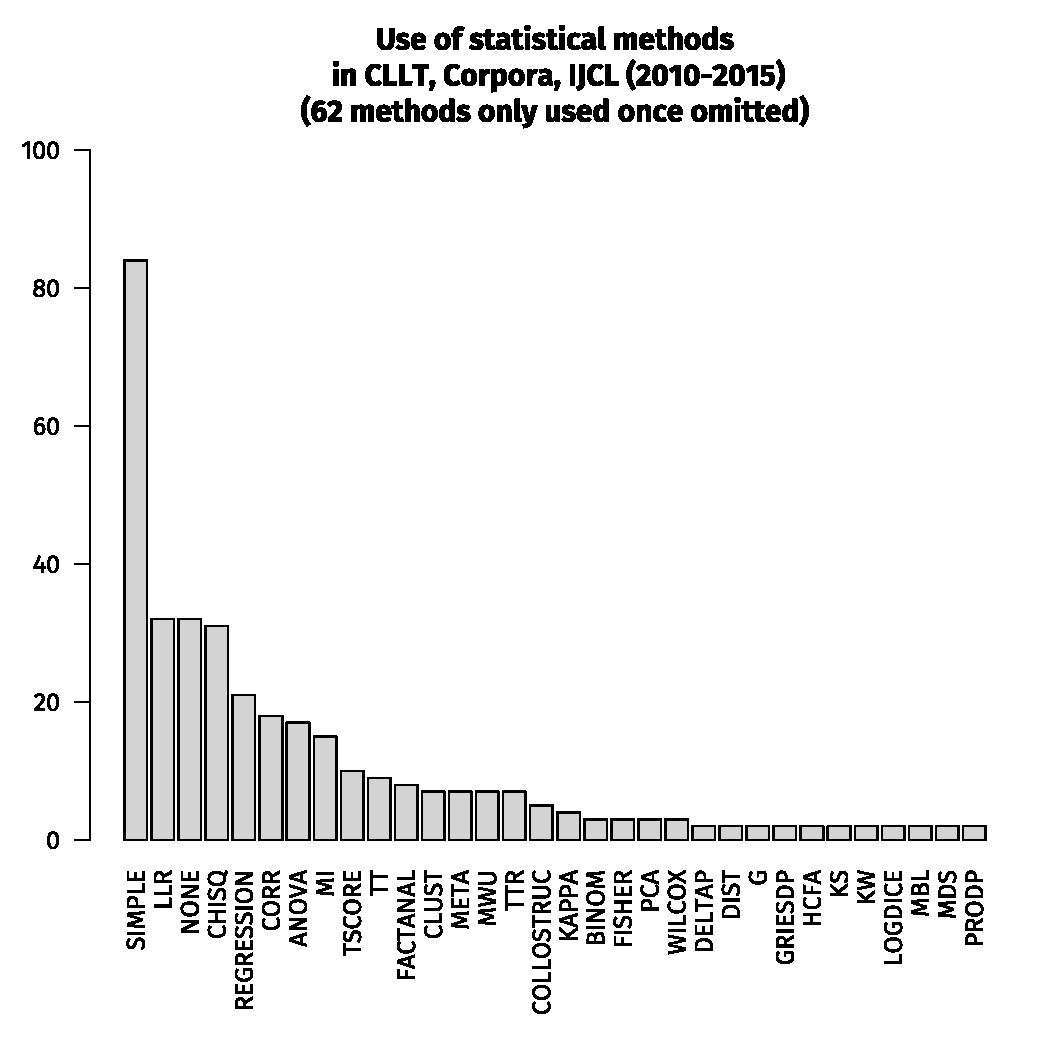
\includegraphics[width=\textwidth]{graphics/statsuse}
  \caption{Use of statistical methods in major corpus linguistics journals; multiple codes per paper were possible; SIMPLE was coded for papers using descriptive statistics, plots, or simple comparisons of relative or absolute frequencies; NONE was coded for papers using no statistics at all; META was coded for methodological papers (in which case individual methods were \textit{not} coded)}
  \label{fig:statsuse}
\end{figure}

With regression models becoming (at least a part of) the state of the art in corpus linguistics, I want to point out that a recent trend to \textit{model everything} might be justified but not strictly required.
First, I provide a brief introduction to regression modelling using binary regression, a highly popular type of regression in the modelling of binary alternations, as an example.%
\footnote{My view on regression and multilevel models is strongly guided by \citet{GelmanHill2006}.
I also use \citet{ZuurEa2009,FahrmeirEa2013,Fox2016} as reference text books.}
Then, I discuss the programme laid out in \citet{Gries2017a}, where a number of factors are enumerated that regression models \textit{should} take into account.

\paragraph{Generalised linear models}

Binary regression (usually logistic regression) models the influence a number of independent variables cumulatively exert on a binary dependent variable.%
\footnote{This short introduction is partially based on \citet{Schaefer2019a}.}
In the regression literature, the independent variables are usually called \textit{regressors} and the dependent variable is called the \textit{response}.
In \ROMeasure, for example, the dependent variable was 0 when the alternant given here as \ref{ex:intro:alternation1}, where the kind-denoting noun (\textit{Wein}) and the measure noun (\textit{Glas}) agree in case, was chosen in the exemplar, and it was 1 when the alternant given here as \ref{ex:intro:alternation2}, where the kind-denoting noun has genitive case, was chosen.

\ex.\label{ex:intro:alternation}
    \ag. Wir trinken [[ein Glas]\Sub{Acc} [guten Wein]\Sub{Acc}]\Sub{Acc}.\\
         we drink a glass good wine \\
         \glt We drink a glass of good wine.\label{ex:intro:alternation1}
    \b.  Wir trinken [[ein Glas]\Sub{Acc} [guten Weins]\Sub{Gen}]\Sub{Acc}.\label{ex:intro:alternation2}

The regression estimates the influence of any number of predictors on the probability that the response is 0 or 1.
The theoretically motivated regressors in this particular study included the case of the measure head noun, the semantic class of the measure noun, lemma frequencies of both the measure noun and the kind-denoting noun, document-level indicators of style, and the type of determiner (cardinal or not) used for the whole NP.
The regressors are thus binary, nominal, and numeric.

Generalised Linear Models all work by assuming that the concrete measurements of the features assumed to influence the outcome are multiplied by \textit{coefficients} which encode the direction (positive or negative) and the strength of each regressor's influence.
Continuing with the above example, if the NP in an exemplar indexed $i$ contains a cardinal determiner, the measurement would be $x^c_i=1$, and the model specification would be such that this term is multiplied by a coefficient $\beta^c$ to yield a numeric quantification of the influence (all other things being equal) on the decision to use either variant.
Thus, the model sub-term for this particular regressor looks like (\ref{eq:model01}).

\begin{equation}
  x^c_i\cdot \beta^c
  \label{eq:model01}
\end{equation}

The sub-terms for all $m$ regressors look the same, and they are added up to form the \textit{linear term}.
Also, the \textit{intercept} $\alpha^0$ is added, which encodes the resulting value when all other regressors are 0 and consequently lead to their corresponding sub-terms being 0.
(\ref{eq:model02}) shows a general form for the linear term with $m$ sub-terms.
The index $i$ indexes the single observations (given sample size $n$, $i\in \{1..n$\}).

\begin{equation}
  \alpha^0+\beta^1\cdot x^1_i+\cdots+\beta^m\cdot x^m_i
  \label{eq:model02}
\end{equation}

The influences on the response variable are thus added up, and they are all assumed to encode a linear relationship.
However, such a linear term can assume arbitrary positive and negative values.
A probability, which is what we want to model, is always in the interval $[0,1]$.
To turn the result of the linear term into a probability, the \textit{link function} is applied to the linear term.
For binary regression, the inverse logit or probit functions are typically used, such that the full model specification looks like the form in (\ref{eq:model03}).

\begin{equation}
  Pr(y=1)=logit^{-1}\left[\alpha^0+\beta^1\cdot x^1_i+\cdots+\beta^m\cdot x^m_i\right]
  \label{eq:model03}
\end{equation}

(\ref{eq:model03}) specifies a model and encodes that the Probability $Pr$ of the response $y$ being $1$ -- or simply $Pr(y=1)$ in mathematical notation -- is given by the inverse logit $logit^1[]$ of the linear term which consists of the overall intercept $\alpha^0$ plus the added up concrete values of each $x_i^j$ multiplied by the corresponding coefficient $\beta^j$, in other words $\beta^j\cdot x_i^j$.
When we specify such a model, we ideally make a theoretical commitment to the factors that drive the choice of the alternants.
Setting up the model is thus the crucial step in going from theoretical considerations to a quantitative analysis.

The job of the so-called \textit{estimator} (a type of algorithm typically implemented in statistics software) is to find the optimal values of all $\beta^j$ given the observations (the annotated sample).
Given these values of the coefficients, the model will predict with the best possible accuracy the probabilities of alternant choices given any assignment of the regressor values.
Ideally, the coefficients would be estimated in a way such that the model predicts each outcome encountered in the sample perfectly.%
\footnote{\Ie\ a probability of 1 would be predicted when the actual outcome was 1, and a probability of 0 would be predicted when the actual outcome was 0.}
This is virtually never the case, and there is always going to be a difference between the predictions and the actual outcomes.
These errors are presumed to follow a specific distribution, which is an assumption underlying the estimation process.
In the case of binary regression, the distribution of errors is assumed to be the binomial, and the model presented here would therefore be called a \textit{binomial generalised linear model with a logit link function}.
Generalised linear models are abbreviated as GLM.%
\footnote{Actually, there is a technical distinction to be made between the logistic regression introduced here, which models probabilities, and a proper binomial GLM, which models counts using a binomial regression.
The difference can be neglected for the present purpose.}

\paragraph{Random effects}

An extension of GLMs are \textit{generalised linear mixed models} (GLMMs) or simply \textit{multilevel GLMs}.
The difference is that GLMMs contain so-called \textit{random effects}.
To understand a random effect, a \textit{random intercept} is the best point of departure.
Any nominal variable like grammatical case or verb lemma or speaker has a certain number of levels.
In the following illustration, $l$ is used to denote this number.
Each level defines a group of exemplars (such as those in the nominative, those with the verb \textit{give}, or those uttered by a specific speaker), and they can therefore be called \textit{grouping factors}.
What happens if we use such a variable as a fixed-effect predictor in a GLM (instead of a random effect in a GLMM) is \textit{dummy coding}.

\begin{table}
  \centering
  \begin{tabular}{llll}
    \toprule
    Actual variable & \multicolumn{3}{l}{Dummy variables} \\
    \textbf{Case}   & \textbf{accusative} & \textbf{dative} & \textbf{genitive} \\
    \midrule
    Nominative      & 0 & 0 & 0 \\ 
    Accusative      & 1 & 0 & 0 \\ 
    Dative          & 0 & 1 & 0 \\ 
    Genitive        & 0 & 0 & 1 \\ 
    \bottomrule
  \end{tabular}
  \caption{Dummy coding of a categorical variable \textit{Case} with four levels, resulting in the three binary dummy variables \textit{accusative}, \textit{dative}, \textit{genitive}}
  \label{tab:dummy}
\end{table}

Dummy coding (or \textit{contrast coding}) is a way of encoding a categorical variable as a number of binary variables.
See Table~\ref{tab:dummy} for an illustration of how German case (a four-way variable) could be dummy coded.
The $l$ levels of the grouping factor are dummy-coded as $l-1$ binary variables.
Since the first of the $l$ levels of the grouping factor is encoded by all dummy variables assuming the value 0, only $l-1$ sub-terms are added to the model, and consequently only $l-1$ coefficients are estimated.
The first level of the actual nominal variable (\textit{Nominative} in the example) is thus \textit{on the intercept} and becomes the reference to which all other levels are compared.%
\footnote{Picking one dummy as a reference level is necessary because otherwise, infinitely many equivalent estimates of the model coefficients exist, as one could simply add any arbitrary constant to the intercept and shift the other coefficients accordingly.
However, the estimator works under the assumption that there is a unique maximum likelihood estimate.}
In such a model, the effect of each grammatical case is treated as a fixed population parameter, and one coefficient is estimated for each dummy case.
In other words, the algorithm which estimates the coefficients for the $l-1$ dummy variables tries to find a fixed value for each of them without taking the variation between them into account.
With many levels, this requires a lot of data, and levels for which only a few observations are available in the data set have very imprecise coefficient estimates with large confidence intervals.

Random intercepts are a way of using grouping factors without dummy coding and by taking the between-group variance into account.
They are not estimates of fixed population parameters (\textit{fixed effects}) but predictions of random variables.
If we treat a grouping factor as a random intercept, we simply let the intercept vary by group (by adding a group-specific constant to the overall intercept), and we give the varying intercepts a distribution instead of estimating $l-1$ coefficients.
This is the relevant difference between a fixed effect and a random effect.
The general model specification with one random intercept looks like (\ref{eq:glmm01}).

\begin{equation}
  Pr(y=1)=logit^{-1}\left[\alpha^0+\alpha^1_{g[i]}+\beta^1\cdot x^1_i+\cdots+\beta^m\cdot x^m_i\right]
  \label{eq:glmm01}
\end{equation}

The only addition compared to (\ref{eq:model03}) is $\alpha^1_{g[i]}$.
I use the notation $g[i]$ (borrowed in a modified form from \citealt{GelmanHill2006}) to indicate that the appropriate $g$-th lemma intercept is chosen for the $i$-th observation.
If, for example, exemplar $9$ contains the verb \textit{give}, which is encoded as group $13$, then $i=9$, and $g[i]=g[9]=13$.
Thus, we now have an intercept which varies by group (instead of one term with its own coefficient per group).
Crucially, instead of estimating a batch of coefficients for the lemma effect, the random effect is itself modeled, and random terms are predicted for each level of the random effect.
For this, the assumption in (\ref{eq:glmm02}) is made.

\begin{equation}
  \alpha_g\sim N(\mu_g,\sigma_g^2)
  \label{eq:glmm02}
\end{equation}

This is standard notation to indicate that the values of $\alpha_g$ follow a normal distribution with mean $\mu_g$ and a variance of $\sigma_g^2$.
In fact, we can regard (\ref{eq:glmm02}) as a minimal second-level linear model already, although one which simply predicts varying intercepts from a normal distribution.
All more complex mixed or multilevel models are extensions of this approach.


\paragraph{Choosing fixed or random effects}

The decision between a fixed (dummy-coded) effect and a varying intercept boils down to two points.
First, the variance in the intercepts needs to be estimated.
Second, the random intercepts can be understood as a compromise between fitting separate models for each group of the grouping factor (\textit{no pooling}) and fitting a model while ignoring the grouping factor altogether (\textit{complete pooling}); see \citet[Ch.~12]{GelmanHill2006}.
As was stated above in (\ref{eq:glmm02}), the random intercepts are assumed to follow a normal distribution, and the variance $\sigma_g^2$ needs to be estimated with sufficient precision.
From the estimated variance and the data, the estimator then predicts the \textit{conditional modes} in GLMMs for each group (see \citealt[Ch.~1]{Bates2010}), which is the numerical value for each group which encodes the per-group tendency.
This procedure, however, requires that the number of groups must not be too low to effectively achieve this.
As a rule of thumb, having fewer than five levels means that a grouping factor should be included as a fixed effect, regardless of its conceptual nature.
Even if there is a default recommendation to use a speaker grouping variable as a random effect, it is ill-advised to do so if there are exemplars from less than five speakers in the sample.
Along the same lines, mode (typically spoken vs.\ written) is no suitable grouping factor for use as a random effect.
Very often, the estimator will simply fail under such conditions, and a fixed effect might be the only option for technical reasons.

If, however, the number of groups is reasonably large, the number of observations per group is the second parameter to consider.
Alternatives to using a random effect would be to estimate a separate model for each level of the grouping factor or to include it as a fixed effect.
If a random effect is used, the conditional modes are \textit{shrunken} (\ie\ pulled) towards the overall intercept.
This is called \textit{shrinkage}.
When the number of observations in a group is low, the conditional mode is shrunken more strongly, and only a small deviation from the overall tendency is predicted for the group.
In such a situation (low numbers of observations per group), fixed effect estimates would turn out to be inexact.
Clearly, low numbers of observations in all or some groups speak against using fixed effects grouping factors.
Random effects are unproblematic under such conditions because of shrinkage.

This purely technical view of fixed vs.\ random effects is not in line with most introductory textbooks written for practitioners.
One commonly given reason for using a random effect instead of a fixed effect is that the researcher is allegedly not interested in the individual levels of the random effect or similar, seemingly conceptual arguments.
It appears that there is little foundation to such claims.
\citet[245--247]{GelmanHill2006} summarise the diverging and contradictory recommendations regarding what should be a random effect as found in the literature.
They conclude that there is essentially no universally accepted and tenable conceptual criterion for deciding what should be a random effect and what a fixed effect.
I agree with them and consider the decision primarily a technical one, \ie\ we use what works best, preferring random effects whenever possible.

\paragraph{Varying intercepts and slopes}

If the coefficients $\beta$ also vary by group, varying slopes are a possible extension of simple GLMs.
We extend the model from (\ref{eq:glmm01}) by giving $\beta^1$ a random slope.
Instead of estimating a fixed coefficient, coefficients are predicted and assumed to come from a random (normal) distribution.
The other fixed effect coefficients remain the same; see (\ref{eq:glmm05}).
We use $\beta^j_{g[i]}$ to denote the coefficient $j$ varying by group $g$, which is chosen appropriately for exemplar $i$.

\begin{equation}
  Pr(y=1)=logit^{-1}\left[\alpha^0+\alpha^1_{g[i]}+(\beta^1+\beta^1_{g[i]})\cdot x^1_i +\beta^2\cdot x^2_i+\cdots+\beta^m\cdot x^m_i\right]
  \label{eq:glmm05}
\end{equation}

A source of problems in varying intercepts and varying slopes (VIVS) models is the fact that in addition to the variance in the intercepts and slopes, the covariance between them has to be estimated.
If in groups with a higher-than-average intercept, the slope is also higher than average, then they are positively correlated, and the reverse applies for lower-than-average intercepts and slopes.
These relations are captured in the \textit{covariance}.
Condition (\ref{eq:glmm06}) is added (the superscript indices on $\alpha$ and $\beta$ have been omitted for readability).

\begin{equation} 
  \left( \begin{smallmatrix} \alpha \\ \beta \end{smallmatrix}\right) \sim
    \left(
    \left( \begin{smallmatrix} \mu_{\alpha}\vphantom{\beta} \\ \mu_{\beta}\vphantom{\beta} \end{smallmatrix} \right), 
      \left( \begin{smallmatrix} \sigma_{\alpha}^2 & \rho\sigma_{\alpha}\sigma_{\beta} \\
	\rho\sigma_{\alpha}\sigma_{\beta} & \sigma_{\beta}^2 \end{smallmatrix} \right)
    \right)
  \label{eq:glmm06}
\end{equation}

(\ref{eq:glmm06}) says that the joint distribution of the intercepts $\alpha$ and the slopes $\beta$ follows a bivariate normal distribution with means $\mu_{\alpha}$ and $\mu_{\beta}$.
The variance in the intercepts is $\sigma_{\alpha}$, the variance in the slopes is $\sigma_{\beta}$, and the coefficient for the covariance between them is $\rho$.
Figure~\ref{fig:multnorm} shows the bivariate density distributions for two (1) negatively correlated, (2) non-correlated, and (3) positively correlated normally distributed variables.

\begin{figure}[!htpb]
  \centering
  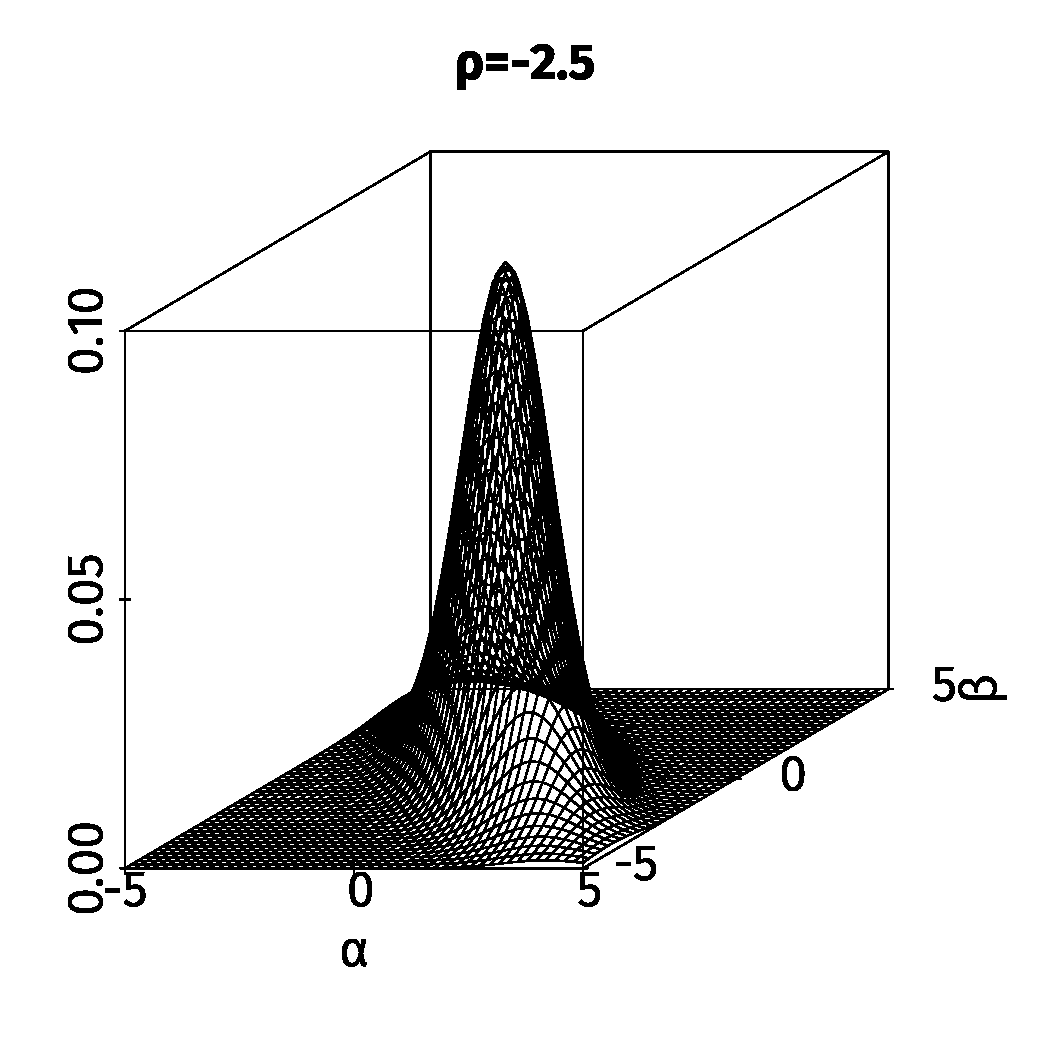
\includegraphics[width=0.33\textwidth]{graphics/multnorm1}~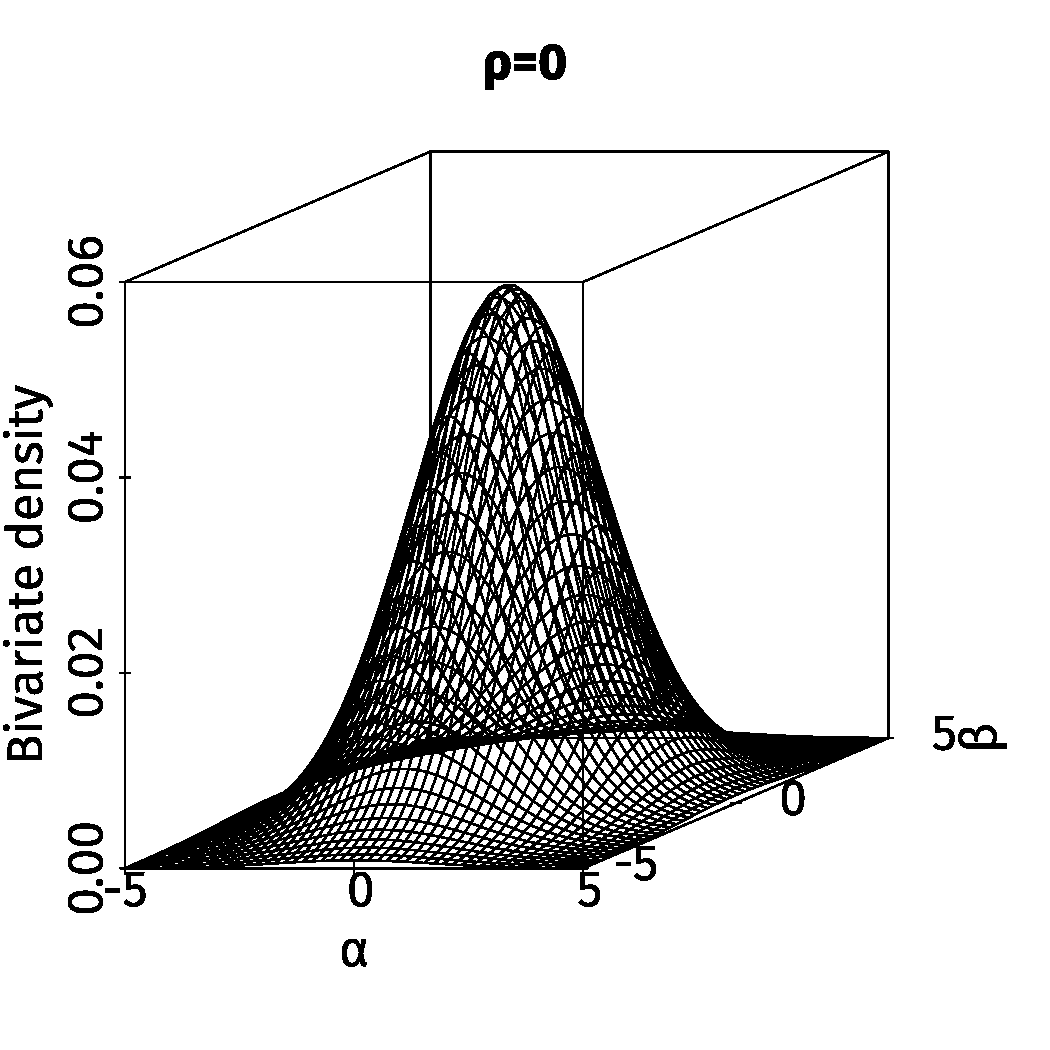
\includegraphics[width=0.33\textwidth]{graphics/multnorm2}~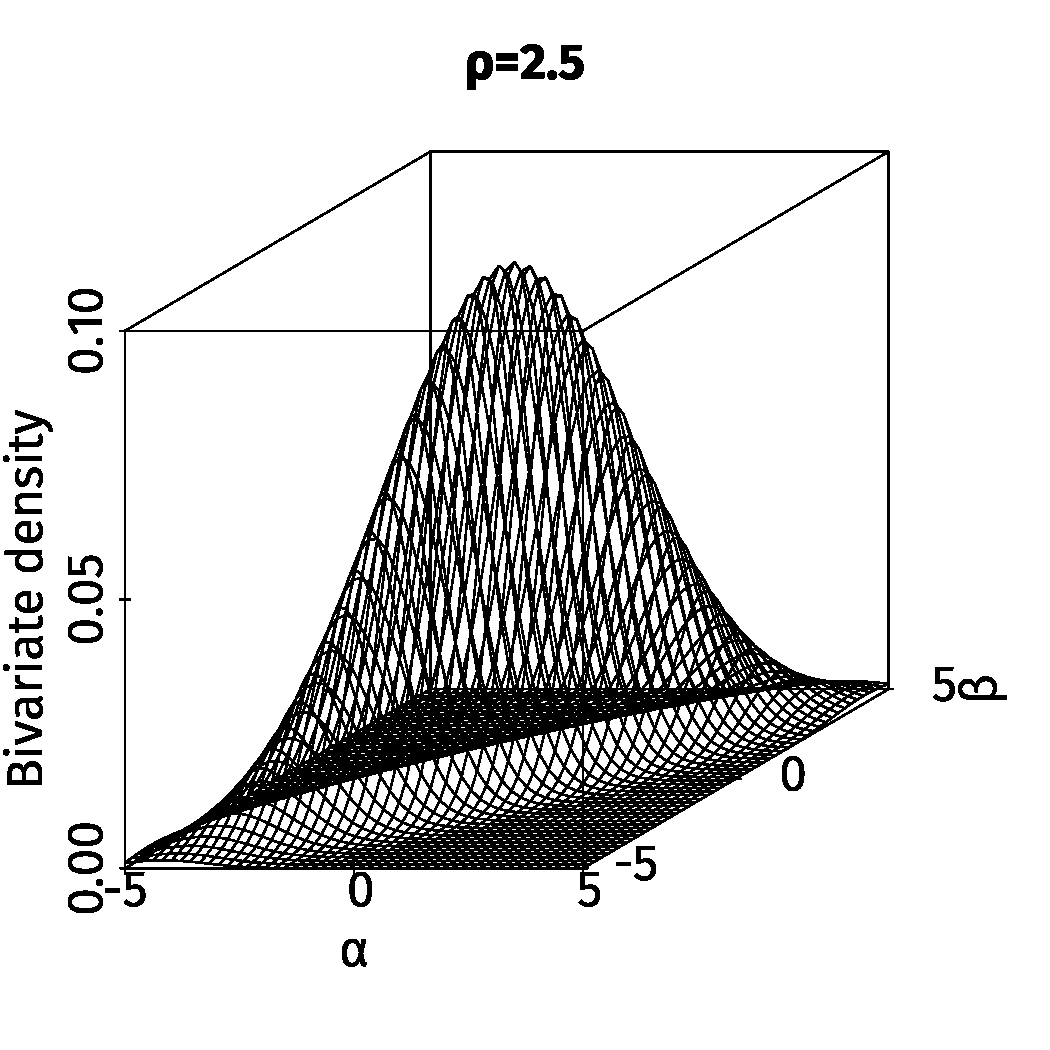
\includegraphics[width=0.33\textwidth]{graphics/multnorm3}
  \caption{Bivariate normal density distribution with different correlation coefficients $\rho$; $\sigma_{\alpha}=\sigma_{\beta}=3$; $\mu_{\alpha}=\mu_{\beta}=0$}
  \label{fig:multnorm}
\end{figure}

The number of variance parameters to be estimated thus obviously increases with more complex model specifications, and the estimation of the parameters in the presence of complex variance-covariance matrices requires considerably more data than estimating a single variance parameter.
The estimator might converge, but typically covariance estimates of $-1$ or $1$ indicate that the data was too sparse for a successful estimation of the parameter.
In this case, the model is \textit{over-parametrised} and needs to be simplified.
See \citet{BatesEa2015a,MatuschekEa2017}.

\paragraph{Second-level predictors}

The linear Gaussian models for random intercepts and slopes can also have fixed-effect regressors themselves (see \RAMeasure\ for an application).
This means that the random effects are partially predicted from a set of separate fixed-effect regressors.
A good example are per-lemma random effects to take care of lemma-specific preferences, but with lemma frequencies, semantic classes of the lemmas, etc.\ being able to partially predict these tendencies.
Thus, the tendencies are not just idiosyncrasies of lemmas, but also determined by properties of the lemma.
In this case, an additional linear model is specified for the random effect instead of the simple normal distribution predictor.
We now extend (\ref{eq:glmm01}) by a predictor $\delta_1$ as a second-level predictor for $\alpha^1_g$.
The first-level model specification remains the same, and it is repeated here as (\ref{eq:glmm08}).

\begin{equation}
  Pr(y=1)=logit^{-1}\left[\alpha^0+\alpha^1_{g[i]}+\beta^1\cdot x^1_i+\cdots+\beta^m\cdot x^m_i\right]
  \label{eq:glmm08}
\end{equation}

However, instead of (\ref{eq:glmm02}), the varying intercept is now predicted from (\ref{eq:glmm09}).

\begin{equation}
  \alpha^1_g\sim N(\gamma^0+\delta^1\cdot u^1_g,\sigma_g^2)
  \label{eq:glmm09}
\end{equation}

Instead of just predicting the mode of each $\alpha^1_g$ value, the model in (\ref{eq:glmm09}) specifies a second-level intercept $\gamma^0$ and a second-level fixed coefficient $\delta^1$, where $u^1_g$ is the value of the second-level regressor variable for group $g$.
True multilevel models increase the complexity of GLMMs, especially if third-, fourth-, or more-level models are used.
Situations for multilevel modeling are quite frequently encountered.
Especially when it comes to speakers as random effects, age, gender, region of birth (if this grouping factor has too few levels to be used as a random effect nesting the speaker random effect), etc.\ are ideal second-level predictors.
The same goes for lemma frequencies, semantic classes, etc.\ as pointed out above.

This short introduction demonstrates that GLMMs or multilevel models can quickly become highly complex.
With increasing complexity, however, more and more data are required for the estimation of the parameters and the predictions of the random variables.
This leads nicely into the final point I want to make in this section.

\paragraph{Modelling everything}

So far, this section has provided a minimal introduction to GLMMs and true multilevel models.
I have shown that models become rather complex relatively easily, and it was pointed out that especially in VIVS models, the necessary estimation of variance-covariance matrices requires a lot of data.
Over-parametrisation in models for experimental data (as touted by \citealt{BarrEa2013}) was heavily criticised by \citet{BatesEa2015a,MatuschekEa2017}.
In a situation of over-parametrisation, it should be noted that even an estimator which is more robust (such as maybe Bayesian estimators) cannot make reliable inferences possible where the data are insufficient given the model's complexity.%
\footnote{Read more comments on Bayesian estimators in Section~\ref{sec:bayesianhype}.}
\citet[1]{BatesEa2015a} state (emphasis is mine): 

\begin{quote}
  We show that failure to converge typically is not due to a suboptimal estimation algorithm, but is a consequence of attempting to fit a model that is too complex to be properly supported by the data, \textit{irrespective of whether estimation is based on maximum likelihood or on Bayesian hierarchical modelling with uninformative or weakly informative priors}.
  Importantly, even under convergence, over-parametrisation may lead to uninterpretable models.
\end{quote}

For corpus-based alternation research, \citet{Gries2017a} argues for massively more complex models compared to the current state of the art (including his own work), and over-parametrisation will certainly occur in many cases.
His line of argumentation follows the previously published \citet{Gries2015}.
In \citet[21--24]{Gries2017a}, he argues that a large number of predictors should be standardly added to alternation models, such as lengths of words and constituents, information-structural predictors, NP types, animacy, and priming\slash persistency predictors, which encode potentially numerous effects of words and constructions which occurred before the target item.
In \citet{Gries2015}, he argues that random effects for text types, speakers, lemmas, etc.\ should also be added as part of the standard protocol (at least whenever the corpus contains the appropriate metadata).
\citet[24]{Gries2017a} admits that

\begin{quote}
  [t]he bad news, as so often, is that this requires an ever increasing or nearly overwhelming degree of sophistication and knowledge not only in linguistics but also in matters of data analysis and statistical evaluation.
\end{quote}

Given that complex models are used in many fields, I would argue that what can be expected of biologists, sociologists, econometricians, etc.\ (or students of these fields) can be expected of linguists, too.
Textbooks at all levels of technicality exist, and \citet{GelmanHill2006} is a true eye-opener which is still accessible for practitioners.
My main practical objection to the model everything approach (MEA) is another one.
Given the complexity of the resulting multilevel models and the fact that a great many of the variables mentioned by \citet{Gries2017a} would have to be annotated manually for any given study, the time and manpower required to conduct even a simple experiment would be disproportional, especially in a competitive academic environment where researchers are pressured to publish several studies each year.
After all, the ideal models under Gries' MEA would very likely require samples containing many tens of thousands of exemplars.

It would be highly frustrating, however, not to implement MEA simply because it is not feasible due to limited resources.
Therefore, I would like to argue that it is often not even necessary for substantive reasons.
MEA is guided by very good reasons, and I will now discuss the two most important ones, interspersed with discussions of why, despite these reasons, this approach may still be unnecessary.
First of all, the goal in alternation modelling might be to model the cognitive representations and processes which make speakers use one form or the other.
In this case, we should indeed add \textit{all relevant causal} predictors available (with emphasis on \textit{all}, \textit{relevant}, and \textit{causal}).
However, unless we have a tight and formally precise theoretical model of these cognitive representations and processes, simply adding everything that we can think of to the model which \textit{might} influence the choice of alternants (even if other studies have produced evidence for such influences under different circumstances) is misguided and prone to producing a significant number of spurious correlations (see Section~\ref{sec:nevereverrandomfallacy}).
This point is strongly related to the limited power corpus data have in making inferences about cognitive representations and processes (see Sections~\ref{sec:prototypesandexemplars} and~\ref{sec:corporaincognitivelyorientedlinguistics}).
In my studies, much like in controlled experiments, I use models which specify a configuration of theoretically motivated predictors, and I do not include any predictors (except sometimes lemma-specific random effects and lemma frequency) for which there is no substantive hypothesis or at least sound previous research.%
\footnote{In \ROMeasure, for example, previous independent theory-driven research by \citet{Zimmer2015} had shown that grammatical case influences the alternation.
Although my own theoretical model did not include case as a predictor, I still added it to increase the quality of the model fit (see below) without risking picking up spurious effects.}
Under MEA, it is even possible that an arbitrary but strong effect masks a substantive and causal effect (see Section~\ref{sec:nevereverrandomfallacy} for a discussion of these terms), and the danger of this happening rises with the number of predictors added to the model on a hunch.
Put differently and more radically, doing a monofactorial study which substantiates the existence of a causal mechanism between a predictor and the alternation might be worth substantially more than estimating a complex model (maybe even with high predictive power) that is not substantive.%
\footnote{Of course, things get significantly worse if a MEA model is taken as evidence for causal mechanisms.
In no way, shape, or form does Gries do this in any of his publications, but other researchers might (implicitly or explicitly).}

The second argument for MEA is that unmodelled variance in a (G)L(M)M has negative effects on the estimator.
Some textbooks like \citet{ZuurEa2009} capitalise on this.
Depending on the severity of this effect, models which are not maximal could actually be wrong, and this argument certainly deserves closer examination.
Two types of situations have to be considered in this regard.
In the first type of situation, an omitted predictor interacts with one or more predictors in the model.
For example, the discourse status of the subject is part of the model specification, but the lemma of the governing verb is not.
However, in reality, the two variables interact, meaning that the strength of the influence of the discourse status is different for different governing verbs.
In this case, the actual coefficient estimates will be different for the predictors which are part of the model specification depending on whether the other regressor (verb lemma in the example) is included or not.
There is no principled solution to this problem, however.
First of all, simply adding all conceivable types of regressors (MEA) and hunting for interactions is, again, just a recipe for finding many spurious effects.
Second, the coefficients might change if some predictor is added, but if its effect and the interaction with another predictor are arbitrary and not motivated (\ie\ causal), then we should not be interested in the \textit{updated} coefficients.
Again, working with substantive models is the solution to this problem.

In the second type of situation, the omitted predictor and the non-omitted predictors do not interact.
In this case, the coefficient estimates for the non-omitted predictors will be stable, \ie\ unaffected.
However, due to excess variance, the estimates of the standard deviations for the fixed-effects coefficients will be different, which is why \citet{BarrEa2013} predict dramatically inflated type I error rates for non-maximal models.%
\footnote{A type I error is a term from the Neyman-Pearson theory of statistical inference, often used in NHST as well.
It occurs when the null is true but rejected by the test.}
This effect is often used to argue for the inclusion of random effects \citep{Gries2015} although it does not matter at all whether the omitted predictors are used as random or fixed effects (see above on the difference).
However, as long as we do not over-parametrise our models, we have so much data that Fisherian tests on fixed effect coefficients are highly sensitive, and p-values for strong effects are mostly extremely low (see all four case studies collected here).
Thus, adapting the standard \textit{sig} level for alternation studies using GLMMs will take care of this problem.
Substantial effects will usually still reach \textit{sig}=0.001, but unmodelled heterogeneity will not cause insubstantial effects to reach \textit{sig}=0.001.
Conversely, with over-parametrised models, \textit{sig}=0.05, and even more data, we run once again the risk of detecting spurious effects and ending up with essentially uninterpretable models \citep{BatesEa2015a,MatuschekEa2017}.

A minor nuisance in the second type of situation is that in GL(M)Ms with a binary response (logit and probit models) unmodelled variance (or \textit{unmodelled heterogeneity}) pulls the coefficient estimates towards 0, which is called the \textit{attenuation bias} \citep[582--585]{Wooldrige2010}.
However, our samples are usually large enough in corpus linguistics (at least -- again and ironically -- as long as we do not over-parametrise the models), and

\begin{quote}
  we should remember that, in nonlinear models, we usually want to estimate partial effects and not just parameters.
  For the purposes of obtaining the directions of the effects or the relative effects of the continuous explanatory variables, estimating $\beta/\sigma$ [the coefficient biased towards 0 through unmodelled heterogeneity; RS] is just as good as estimating $\beta$ [the true coefficient; RS].

  To be more precise, the scaled coefficient, $\beta_j/\sigma$, has the same sign as $\beta_j$, and so we will correctly (with enough data) determine the direction of the partial effect of any variable -- discrete, continuous, or some mixture -- by estimating the scaled coefficients. \citep[583]{Wooldrige2010}
\end{quote}

Thus, it will be harder to detect an effect if there is a significant attenuation bias, but we will still make very similar inferences given enough data.

To summarise, I have argued for well-specified, non-maximal models and against MEA.
The dangers of uninterpretable over-parametrised models which attempt to model many more effects than the amount of data is appropriate for by far outweigh the risks of omitted regressors or unmodelled variance.
Furthermore, MEA might lead to many spurious effects being included in models, and thus probably being taken seriously.
Instead, I argue for model specifications grounded in substantive theory and previous research.
If such types of model specifications are difficult to come up with, I suggest the field invest more time and resources into producing powerful, highly predictive, and formally specified theories instead of engaging in data dredging.


\subsubsection{Just go Bayesian?}
\label{sec:bayesianhype}

In this section, I justify the choice of statistics which I used in all my studies collected here, namely non-Bayesian statistics.
Over the past few years, modified versions of or alternatives to (multilevel) generalised linear models with a Maximum Likelihood Estimator (MLE) have been proposed.
From among these methods, I just make a few remarks on Bayesian estimation (see \citealt{GelmanEa2014}) as it was proposed in \citet{Levshina2016} and \citet{Divjak2016a}, for example.
Conceptually, I see three points of discussion that should be kept apart.
First, Bayesian methods are sometimes touted as superior tools for scientific inference compared to frequentist methods.
Second, it has been proposed that the Bayesian interpretation of probability is more cognitively adequate for the modeling of linguistic data \citep[301--302]{Divjak2016a}.
Third and very specific to this paper, given the established methods in the modeling of alternation and variation, it has to be decided whether so-called Bayesian methods lead to substantially different results.

As for the first point, the relevant fundamentals of frequentism have already been mentioned in Section~\ref{sec:onstatisticalinference}.
The basic distinction between frequentism and Bayesianism is a philosophical one and related to the concepts of \textit{direct} and \textit{inverse probability} (\eeg\ \citealt{Senn2011}).
Frequentists assume that models and parameters are fixed and given by theories, for example a model specifying that a coin is fair.
We can then calculate for observed data (for example a measurement of three heads in an experiment with ten tosses) how often such a result or a more extreme result would occur if the model were true and if we repeated the experiment arbitrarily often.
This is essentially the frequentist notion of direct probability, \ie\ long-run frequencies under replication.
Standard tests in the Fisher and Neyman-Pearson traditions as well as Neyman confidence intervals are based on this concept of probability.
Bayesian approaches (in the now common interpretation), on the other hand, are conditioned on the particular data and quantify inductively the probability of model parameters given the available data.
The parameters are thus not fixed, and the resulting probability is usually equated with researchers' posterior beliefs about model parameters.
The problem is that researchers often need a criterion that tells them whether a hypothesis was substantiated by an experiment or not (hypothesis testing and error control).
There is actually a debate among Bayesians about the proper interpretation of Bayesian methods and whether a notion of hypothesis testing is compatible (or even already contained) in the Bayesian approach.
In \citet[10]{GelmanShalizi2013}, the authors -- prominent Bayesians themselves -- acknowledge that a theory of statistical testing is a desideratum, state about the standard inductive interpretation of Bayesianism that ``most of this received view of Bayesian inference is wrong'', and develop a Bayesian notion of p-values (see also \citealt{Mayo2013}, for a frequentist reply; also \citealt{Senn2011} on different strands of Bayesianism and their stance on inductive vs.\ deductive reasoning, and \citealt{Mayo2011}, for a critical reply to \citealt{Senn2011}).
Clearly, in such quarrels between and among camps of science philosophers and statisticians, it is difficult for mere practitioners to take sides.

Turning to the second point, \citet[301--302]{Divjak2016a} speaks favourably of Bayesian methods because the Bayesian concept of probability is allegedly better-suited for cognitive modelling than the frequentist one.
Her argument is part of a larger body of literature asking for cognitively plausible modelling techniques, for example Naïve Discriminative Learning (NDL; \citealt{Baayen2011,BaayenEa2013,MilinEa2016,TheijssenEa2013}).%
\footnote{On p.\ 303 of \citet{Divjak2016a}, the author goes on to explicitly mention NDL as well.}
Yet, neither frequentist nor Bayesian methods were conceived of as cognitive models, but as systems of inference for scientists (see above, and see also \citealt[302]{Divjak2016a}).
The fundamental question that lurks behind such arguments is how we interpret our statistical models (estimated on corpus data).
Are they inductive models of cognitive representations which human learners would also infer through being exposed to the corpus data?%
\footnote{In which case we would be doing \textit{data science in language research} in the words of \citealt{MilinEa2016}.
I see this as standing in contradiction to the view advocated in \citet{Dabrowska2016} as cited above (p.~\pageref{abs:dabrowska}).}
Or are they tests of theories that are pre-specified and merely tested for predictive accuracy on linguistic output data contained in corpora?
In the former case, we adopt a strong \textit{corpus as input} hypothesis \citep{StefanowitschFlach2016} and should maybe resort to cognitively plausible statistical methods (whatever these might be).
In the latter and less extreme case, the cognitive commitment does not necessarily extend to the statistical methods used.
These methods, then, do not need to be any more cognitively plausible than an ANOVA used to analyse the results from an experiment in cognitive science.
I view my own work in the tradition of theory testing, and cognitive realism is thus not a requirement for my methods of statistical inference of choice.

With regard to the third point, \citet[251--252]{Levshina2016} argues for Bayesian estimation in mixed regression settings.
First, she claims that ``while frequentist statistics only allows one to test whether the null hypothesis can be rejected, Bayesian statistics enables one both to test the null hypothesis and to estimate the probability of specific parameter values given the data''.
This does not do justice to frequentist methods (and makes it sound like the author equates frequentism with NHST) in that mere rejection of the null hypothesis is characteristic only of Fisher's approach in its most rudimentary version.
In the Neyman-Pearson approach, results actually \textit{favour} one hypothesis over the other (cf.\ \citealt{Lehmann1993,Lehmann2011,Perezgonzalez2015}) and lead to informed decision making.
Furthermore, especially Neyman-style frequentism has well-known extensions to estimation, for example in the form of confidence intervals (see \citealt{GreenlandEa2016}, esp.\ p.\ 340).
Levshina then also explains that a ``distinctive feature of Bayesian statistics is the use of so-called priors'' and that ``posterior probabilities depend on both the prior beliefs and the data, whereas the results of a frequentist model depend only on the data'' \citep[252]{Levshina2016}.
Remarkably given this statement, she does \textit{not} use informative priors, and in her footnote 8, \citet[252]{Levshina2016} admits that priors were probed using trial and error.
So, the proclaimed major advantage of Bayesian modeling was apparently not taken advantage of.%
\footnote{In the words of \citet{Senn2011}: ``You may believe you are a Bayesian but you are probably wrong.''
Even \citet[347--348]{GelmanHill2006} ``view any noninformative prior distribution as inherently provisional'' and give recommendations how to proceed once posteriors have been obtained from noninformative priors.}

\begin{sidewaystable}
  \centering
  \resizebox{\textheight}{!}{
  \begin{tabular}{llrlp{0.5em}rrp{0.5em}rrp{0.5em}rrp{0.5em}cc}
      Level & Regressor & \multicolumn{1}{l}{\pPB} & Level  && \multicolumn{2}{l}{Coefficient} && \multicolumn{2}{l}{CI low} && \multicolumn{2}{l}{CI high} && \multicolumn{2}{l}{CI excludes 0} \\
              &                   &       &           && \multicolumn{1}{l}{MLE} & \multicolumn{1}{l}{MCMC} && \multicolumn{1}{l}{MLE} & \multicolumn{1}{l}{MCMC} && \multicolumn{1}{l}{MLE} & \multicolumn{1}{l}{MCMC} && \multicolumn{1}{l}{MLE} & \multicolumn{1}{l}{MCMC} \\\midrule
       First     & Badness           &  0.002 &           && -0.152 & -0.155 && -0.247 & -0.247 && -0.061 & -0.065 && * & * \\
                 & Cardinal          &  0.001 & No        &&  1.189 &  1.222 &&  0.862 &  0.927 &&  1.466 &  1.496 && * & * \\
                 & Genitives         &  0.001 &           && -0.693 & -0.711 && -0.768 & -0.801 && -0.592 & -0.616 && * & * \\
                 & Measurecase       &  0.001 & Acc       &&  0.030 &  0.031 && -0.150 & -0.159 &&  0.212 &  0.222 &&   &   \\
                 &                   &        & Dat       &&  0.705 &  0.729 &&  0.455 &  0.465 &&  0.944 &  0.995 && * & * \\[0.5\baselineskip]
       
       Second    & Kindattraction    &  0.020 &           &&  0.225 &  0.244 &&  0.049 &  0.056 &&  0.393 &  0.422 && * & * \\
       (Kind)    & Kindfreq          &  0.095 &           &&  0.146 &  0.164 && -0.023 & -0.016 &&  0.301 &  0.341 &&   &   \\
                 & Kindgender        &  0.001 & Neut      &&  0.021 &  0.013 && -0.367 & -0.409 &&  0.392 &  0.435 &&   &   \\
                 &                   &        & Fem       &&  1.269 &  1.289 &&  0.800 &  0.788 &&  1.709 &  1.783 && * & * \\[0.5\baselineskip]
       
       Second    & Measureattraction &  0.001 &           &&  0.282 &  0.299 &&  0.106 &  0.102 &&  0.447 &  0.515 && * & * \\
       (Measure) & Measureclass      &  0.001 & Container &&  0.252 &  0.257 && -0.265 & -0.303 &&  0.788 &  0.813 &&   &   \\
                 &                   &        & Rest      &&  0.421 &  0.379 && -0.209 & -0.378 &&  1.063 &  1.091 &&   &   \\
                 &                   &        & Amount    &&  0.831 &  0.889 &&  0.215 &  0.220 &&  1.432 &  1.569 && * & * \\
                 &                   &        & Portion   &&  1.217 &  1.253 &&  0.675 &  0.689 &&  1.684 &  1.840 && * & * \\
                 & Measurefreq       &  0.005 &           && -0.231 & -0.232 && -0.363 & -0.395 && -0.079 & -0.073 && * & * \\

  \end{tabular}
  }
  \caption{For the main study from \ROMeasure: coefficient table comparing Maximum Likelihood Estimation (MLE, with 95\% bootstrap confidence interval; 1,000 replications) and Bayesian Markov-Chain Monte Carlo estimation (MCMC; 4 chains; 1,000 iterations; normal priors for coefficients); the intercept (\textit{Cardinal=Yes}, \textit{Measurecase=Nom}, \textit{Kindgender=Masc}, \textit{Measureclass=Physical}; 0 for all numeric z-transformed regressors) is -3.548 (MLE) and -3.700 (MCMC)}
  \label{tab:bigtable}
\end{sidewaystable}

Now, Maximum Likelihood Estimation (MLE) -- the traditional method which could have been used instead of a Bayesian estimator -- is not inherently \textit{frequentist} in the sense of Neyman-Pearson testing theory.
MLE, like inductive Bayesianism, conditions on the particular data inasmuch as it searches for the most likely set of parameters given the data.
Frequentist testing theory is then used to make inferences based on variance parameters estimated by the ML estimator.
What is more, Bayesian estimators are in fact based on the Likelihood and merely multiply it by the prior \citep[6--8]{GelmanEa2014}.
If the prior is flat, results between MLE and Bayesian estimators converge (see also \citealt[347]{GelmanHill2006}).
The same is true if the sample size is large compared to the number of parameters, at least for finite-dimensional parameter models \citep[1119--1120]{Freedman1999}, a well-established result known as the \textit{Bernstein-von Mises theorem}.
With a modest model structure including 17 fixed effects and 2,646 data points in \citet{Levshina2016}, it is highly likely that the same results would have been obtained with MLE.
In fact, she admits that changing the priors did not lead to substantially different results in her footnote 8.
This is a clear sign that the prior is ``swamped by the data'' \citep[1119]{Freedman1999}.
So far, I see no theoretically well-founded or practical arguments in favour of the Bayesian approach.
If there had been evidence in Levshina's study that Bayesian and MLE methods did \textit{not} converge, it would have been an occasion to demonstrate the selective superiority of the algorithms used in Bayesian estimation.
After all, there are situations where Bayesian estimators can be more robust, namely with heavily censored data, complex hierarchical models, perfect separation, etc. (see \citealt{Freedman1999}, \citealt[345--348]{GelmanHill2006}).

I want to state clearly that these points do not in any way invalidate the results presented in \citet{Levshina2016}.
However, being ``Bayesian'' (as touted in the title of the paper) is most likely not among its selling points.
Additionally, I want to voice the concern that many practitioners are probably already struggling with getting an adequate grasp of advanced statistical methods and that it might therefore be wise to use the more conservative and better understood method if the alternative method is not absolutely required for substantive reasons.

\begin{figure}[htpb]
  \centering
  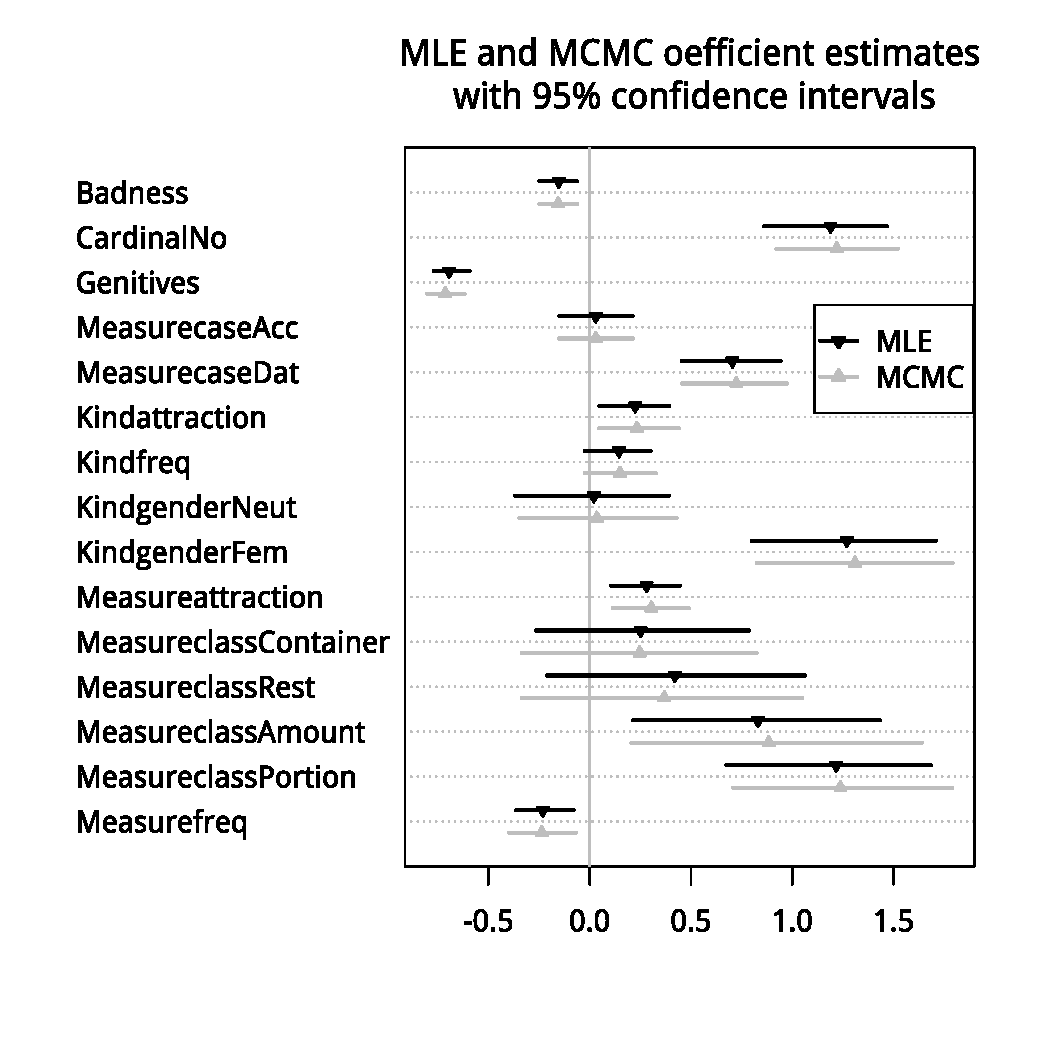
\includegraphics[width=\textwidth]{graphics/corpus_fixeffs_mle+mcmc}
  \caption{For the main study from \ROMeasure: coefficient plot comparing Maximum Likelihood Estimation (MLE, with 95\% bootstrap confidence interval; 1,000 replications) and Bayesian Markov-Chain Monte Carlo estimation (MCMC; 4 chains; 1,000 iterations; normal priors for coefficients); the intercept (\textit{Cardinal=Yes}, \textit{Measurecase=Nom}, \textit{Kindgender=Masc}, \textit{Measureclass=Physical}; 0 for all numeric z-transformed regressors) is -3.548 (MLE) and -3.700 (MCMC)}
  \label{fig:fixeffs}
\end{figure}

Finally, in order to demonstrate the convergence of the two types of estimators, I estimated the parameters of the hierarchical model presented in \ROMeasure\ with MLE and Markov-Chain Monte Carlo (MCMC) methods (the currently most prominent estimator used in Bayesian settings) to demonstrate their expectable convergence.
Table~\ref{tab:bigtable} and the fixed effects coefficient plot in Figure~\ref{fig:fixeffs} show the results.

This concludes the theoretical and methodological evaluation.
I have defended the general approach to alternation modelling and probabilistic grammar, motivated the choice of data (mostly web corpora), and argued that the methods of statistical inference used in my research are indeed valid.
In Section~\ref{sec:casestudies}, I now put the four case studies into perspective before pointing to possible future research in Section~\ref{sec:futuredirections}.


\newpage

\section{Case studies}
\label{sec:casestudies}

In this section, I introduce the four case studies presented in detail in the published papers.
I briefly describe the phenomenon under investigation in each paper, the assumed theoretical models, the methods used, and the paper's contribution to the research in probabilistic modelling and\slash or alternation modelling.
In addition to these contributions, all papers represent innovation and advancement for the grammatical description of German, especially with a focus on non-standard written language and so-called \textit{Zweifelsfälle} `cases of doubt'.
Should a large corpus-based descriptive grammar of German (which should obviously include alternations in its descriptions) ever be written, the studies presented here could serve as a blueprint for such a product.
The details of the painstaking work (data collection, annotation, and fine-grained statistical analysis) reported in each individual paper demonstrate, however, that such an undertaking would be a monumental one lasting decades and requiring substantial manpower.

All studies used the DECOW web corpus \citep{SchaeferBildhauer2012,Schaefer2015b}, which contains a mix of standard and non-standard written German as its main source of data (see Section~\ref{sec:webcorpora}).
The statistics in each paper were programmed in the R programming language \citep{R}.

\paragraph[Graphemic words and new paradigms]{Graphemic words and new paradigms: the cliticised indefinite article}
\mbox{}\\[0.5\baselineskip]\noindent
In \RODefArt, we show how the emerging short forms of the German indefinite article create a new alternative paradigm, thus representing an independent alternative to the full forms.
While the full standard forms use the stem \textit{ein}, the stem is reduced to \textit{n} in the short forms.
The picture is complicated by forms like \textit{nen}, which look like short forms of \textit{einen} (accusative masculine singular), but which are also used as short forms corresponding to \textit{ein} (nominative masculine\slash neuter singular).
We argue that such forms have undergone a reconstruction process to fulfill both phonological and graphemic constraints on independent words.
The paper reports five independent corpus studies.
Study 1 shows that there is some amount of free variation, substantiated by the occurrence of a significant number of exemplars with one short form and one full form in NP conjunction structures with \textit{und} `and' or \textit{oder} `or' (regardless of the case of the NP and the order of the two conjuncts).
Study 2 shows that the overall tendency of not using the genitive in non-standard documents alone does not account for the fact that the paradigm of the short forms does not have a genitive at all.%
\footnote{The expected genitive forms \textit{nes} and \textit{ner} virtually do not occur.}
Study 3 presents a GLM which predicts the alternation between full and short forms using a number of theoretically motivated regressors, the main result being that the masculine and neuter nominative as well as the neuter accusative have the strongest tendency to preserve the full form, which was among the theoretically motivated predictions.
Study 4 shows (using another, much simpler GLM) that the form \textit{nen} is most likely preferred under certain morphophonological and graphemic conditions and not specifically marked for a morphosyntactic function.
Finally, Study 5 shows that independent graphemic principles guide writers' behaviour, as full graphemic enclisis (contraction of the reduced indefinite article with the preceding word without space or apostrophe) occurs predominantly with the form \textit{n}.
This, we argue, can only be explained by the fact that \textit{n} is not at all a prototypical independent graphemic word.

This paper is written in a descriptive tone, not making claims about cognitive representations.
However, since general principles (such as universal and language-specific conditions on enclisis) are referred to, a cognitive interpretation and an experimental cross-validation would be possible.
The paper fits well into the alternation research paradigm, as other studies have been presented within it which also model choices between full forms and contracted (or cliticised) forms, \eeg\ \citet{BarthKapatsinski2014}.
We explicitly argue for the benefits of using web corpora (DECOW12 in this case), because the short forms are entirely absent from standard written language.

\paragraph[Prototypes and paradigms]{Prototypes and paradigms: the strength of weak nouns}
\mbox{}\\[0.5\baselineskip]\noindent
In \ROWeakN, I demonstrate how robust corpus-based models can be constructed and verified based on previous substantive prototype-theoretical research.
The approximately five hundred masculine weak nouns in German like \textit{Mensch} `human, man' follow a remarkably odd inflectional paradigm compared to all other nouns.
They mark all forms except for the nominative singular with \textit{-en}.
While there is another paradigm of masculine\slash neuter nouns which mark the plural with \textit{-en}, the weak singular forms in the accusative, dative, and genitive are truly exceptional.
Furthermore, there is a non-standard alternation inasmuch as weak nouns sometimes occur in strong forms.
If that happens, they simply drop the \textit{-en} in the accusative and dative, and they take on the typical strong ending \textit{-es} instead of \textit{-en} in the genitive.
From \citet{Thieroff2003} -- an analysis of the relevant paradigm structure -- I predict that the strong forms of weak nouns should be more frequent in the accusative and dative than in the genitive.
Base on the prototype-theoretical analysis in \citet{Koepcke1995}, I also predict that the strong forms should be less frequent when the nouns denote humans and when certain phonotactic conditions are met.%
\footnote{Koepcke shows (among other things, based on diachronic data) that the weak nouns predominantly represent a semantically and phonotactically well-defined prototype.
The features enumerated in his paper and used in my model are slightly more fine-grained than this short introduction makes them sound.}
The predictions are borne out in a large-scale corpus analysis using a GLM to predict the alternants.

Obviously, the paper fits well into the alternation modelling approach.
It uses a cognitively motivated model (based on prototype theory) and all the standard tools described in Section~\ref{sec:theoriesmethodsanddata}.
In the future, a re-analysis using a per-lemma random effect will be attempted.
As it stands, lemma-specific effects are not modelled because the estimator did not converge with random effects in the model.
Since new algorithms and statistical packages are constantly being made available, a more realistic statistical model might be possible in the future.

\paragraph[Prototypes and grammaticalisation]{Prototypes and grammaticalisation: the measure NP alternation}
\mbox{}\\[0.5\baselineskip]\noindent
In \ROMeasure, I model a case alternation in German measure noun phrases such as \textit{ein Fass reines Öl} (both nouns have identical case) or \textit{ein Fass reinen Öls} (the kind-denoting noun has genitive case), both `a barrel of pure oil'.
I describe the prototypical meanings of both alternants in terms of the grammaticalisation paths leading to partitive and pseudo-partitive \citep{Koptjevskaja2001} constructions.
Basically, the genitive construction is assumed to prototypically allow both a referent of the measure noun and of the kind-denoting noun to be accessible.
The same is possible but less prototypical for the case identity construction.
From the definition of the prototypes, a number of predictions are derived regarding the preferences of measure nouns from different semantic classes to occur in one alternant or the other.
Also, a prediction regarding cardinal or non-cardinal determiners is derived from the prototypical meanings.

Furthermore, an exemplar effect is modelled.
For the alternating construction, there exist two neighbouring construction which always require the genitive (`ein Fass des reinen Öls' with a determiner on the kind-denoting noun) or never allow the genitive (`ein Fass Öl' with no determiner and no adjective).
The occurrence frequencies of measure and kind lemmas in these two constructions is shown to influence the alternation in the expected direction.

The study is a prime example of corpus-based alternation research based on substantive theory.
Not only is each predictor in the multilevel model independently motivated, but there is also experimental cross-validation in two experimental paradigms (forced choice and self-paced reading).
The paper makes significant contributions to the prototype vs.\ exemplar debate, and it discusses the question of how well corpus-derived models and experimental validations can be expected to converge.

\paragraph[Prototypical syntax and punctuation]{Prototypical syntax and punctuation: (non-)embedded V2 clauses}
\mbox{}\\[0.5\baselineskip]\noindent
Finally, in \ROWeil, Ulrike Sayatz and I use graphemic data from non-standard written German to substantiate conclusions about sentential structure in embedded and non-embedded clauses introduced by the particles \textit{obwohl} `although, then again' and \textit{weil} `because'.
Both particles are subordinators in standard written German and as such embed clauses with verb-last constituent order.
It has been known for quite a while that with some semantic and pragmatic changes they can also embed verb-second clauses, which is the constituent order otherwise typical of independent clauses.

We perform an in-depth analysis of the punctuation occurring before and after the two particles, also using GLMs.
The results are very strong and could even have been detected with descriptive statistics alone.
It turns out that \textit{obwohl} with verb-second order occurs proportionally more often at the beginning of sentences after full stops.
Also, \textit{obwohl} is separated more often from the clause it embeds by punctuation marks which are otherwise used with sentence-initial, verb-second-embedding discourse particles such as \textit{natürlich} `naturally' of \textit{klar} `of course'.
In line with previous research, we argue that the distribution of the punctuation marks provides solid evidence that the two particles (with verb-second order) have different syntactic and pragmatic functions and that \textit{obwohl} is essentially a discourse particle used in independent sentences.

The paper does not straightforwardly belong into the alternation research category, but it clearly models a probabilistic phenomenon, as the syntactic structures, the pragmatic functions, and the graphemic markers are subject to stochastic variation.
The major contribution of the paper is the first-ever proposal of \textit{usage-based graphemics} (UBG).
We understand UBG neither as a theory nor as a framework.
Rather, we see it as a method of analysing graphemic variation as a cue to grammatical structure.
It is a method of analysis which has the potential to develop into a framework concerned with the syntax-graphemics interface.

We assume that writers learn to associate phonological, morphological, and syntactic patterns with graphemic patterns through repeated exposure to the graphemic patterns in conjunction with the grammatical ones.%
\footnote{Despite some construction terminology used in our paper, UBG is not necessarily tied to construction grammar or any other grammatical framework.
Any system of units of grammar and their combinatorics can be mapped onto graphemic patterns.}
Thus, they learn to associate grammatical prototypes (such as sentence type prototypes) probabilistically with graphemic units and patterns such as punctuation marks.
This is clearly in line with assumption of usage-based theories \citep{BybeeBeckner2009}.
Especially when the normative pressure is low (as is the case when, for example, German writers start using the completely non-standard \textit{obwohl} and \textit{weil} clauses with verb-second order in writing) and writers have to encode syntactic structures which are novel or usually not encoded at all in writing, the prototypical mapping becomes visible through emerging regularities where no normative rules exist.

What is promising about this approach is that -- once it is fully developed -- it can be used to reconstruct evidence for grammatical structure from corpora containing non-standard writing.
For this to work reliably, the correspondences and mechanisms have to be fleshed out, and experimental validation is required.
Therefore, it was vital that the results converged with previous analyses of the two particles, thus substantiating the assumption that UBG is a valid method of analysis.
UBG will be described in more detail in \citet{SchaeferSayatz2019} and several other publications by Ulrike Sayatz and me which include experimental work.


\newpage

\section{Future directions}
\label{sec:futuredirections}

My and my co-author's research collected here shows that German has a wide range of phenomena to offer for examination under a usage-based probabilistic perspective.
Furthermore, in the form of the DECOW corpus, a now-proven source of data exists which allows researchers to work on these phenomena.
Based on the argumentation in Sections~\ref{sec:probabilisticgrammar}--\ref{sec:casestudies} and the case studies, a number of open research questions come to mind.
I see at least the following ones.

\vspace{\baselineskip}

\begin{itemize}
  \item The literature on \textit{cases of doubt} in German is famously rich.
    It would be beneficial for linguists working on German, corpus linguists, and linguists working in the cognitively oriented\slash usage-based tradition to examine them using the framework established here.
  \item The effects of corpus composition and the availability of metadata on corpus samples and sampling procedures should be examined further.
    The BNC is rich in metadata and has a well-planned composition, but for many other languages (like German), similar corpora do not exist.
  \item Related to the last point, corpora containing non-standard writing should be honoured more as a unique source of data.
    While there is a community working on such corpora and specific analyses of their content, many more (corpus) linguists could benefit from using them in the same way I did.
  \item Also related to this point, the usage-based perspective on graphemics as developed by Ulrike Sayatz and me should be developed and expanded further.
    Speakers' writing behaviour provides important clues to how they cognitively represent morphological and syntactic categories.
  \item Individual grammatical differences urgently require more attention.
    While it will probably be impossible to build large enough general-purpose corpora with speaker metadata which would allow research on individual grammatical differences, corpus data should be correlated with the reactions of individual speakers in controlled experiments.
  \item The prototype vs.\ exemplar debate would benefit from more large-scale corpus studies which must then be cross-validated in controlled experiments.
    Corpus data alone cannot provide evidence for or against one theory or the other.
  \item Statistical methods need to be scrutinised.
    While mindless applications of NHST are detrimental for valid scientific inferences, some critiques of frequentist statistics (language is never random; model everything) have gone too far or are understood in a much too unrestricted manner.
    Also, some currently-hyped alternative methods do not lead to substantially different results, are understood even less than traditional methods, and distract from the real problems with statistical inference.
\end{itemize}

\vspace{\baselineskip}

Clearly, my work has contributed to all of these points, but the overall situation in probabilistic, usage-based, cognitively oriented corpus linguistics is one where methods and theories are still in a very early stage of development.


\newpage

\printbibliography

\end{document}
